


\documentclass[conference,twocolumn]{IEEEtran}
\usepackage{blindtext, graphicx}
\usepackage{amstext}
\usepackage{caption}
\usepackage{float}
\usepackage{subfigure}
\usepackage{listings}
% correct bad hyphenation here
\hyphenation{op-tical net-works semi-conduc-tor}


\begin{document}
%
% paper title
% can use linebreaks \\ within to get better formatting as desired
\title{Your Flowchart Secretary: Real-Time Hand-Written Flowchart Converter}



\author{
\IEEEauthorblockN{
Qian Yu\IEEEauthorrefmark{1},
Rao Zhang\IEEEauthorrefmark{2}, 
Tien-Ning Hsu\IEEEauthorrefmark{3},
Zheng Lyu\IEEEauthorrefmark{4}
}
\IEEEauthorblockA{Department of Electrical Engineering\\
\{\IEEEauthorrefmark{1}qiany,
\IEEEauthorrefmark{2}zhangrao,
\IEEEauthorrefmark{3}tiening,
\IEEEauthorrefmark{4}zhenglyu\} @stanford.edu}
}

% make the title area
\maketitle

\IEEEpeerreviewmaketitle


\section{Introduction}
Often when we are prototyping new ideas, a flowchart will be an ideal way to explicit our thoughts. However, it could be super time consuming to draw up a well-organized one onto our documentation files or presentation. In that sense, it would be really convenient if we can automatically generate the flowchart template with proper order informed from hand drawing chart. Here we developed an Android implemented application that can generate electronic version when scanning the flowchart. The application can be applied in many settings from discussion and notes in daily use to formal meetings in company or education institution. In addition, this product will be implemented in Android device for users’ convenience.

\section{Related Works}
    Off-line interfaces is early common path to deal with handwritten flowchart problems. A method based on recognizing hand-drawn architectural symbols was discussed in~\cite{valveny1999}. The method operated on 300 dpi bitmaps. Their method realized a 85\% recognition rates. Ramel, et.~al proposed another approach to recognize handwritten shapes by using OCR system~\cite{Ramel1999}.
    
    CLEF-IP competition rises the attention to flowchart recognition since 2012~\cite{Morzinger2012}. Rusiñol, et.~al present a flowchart recognition method aimed at achieving a structured representation of flowchart in CLEF-IP 2013~\cite{Rusinol2014}. The principal approach (as shown in Fig \ref{fig: RW1}) for these work is to retrieve the structure with the nodes of the arrows or the end of lines.
    
\begin{figure}[!htbp]
  \center
  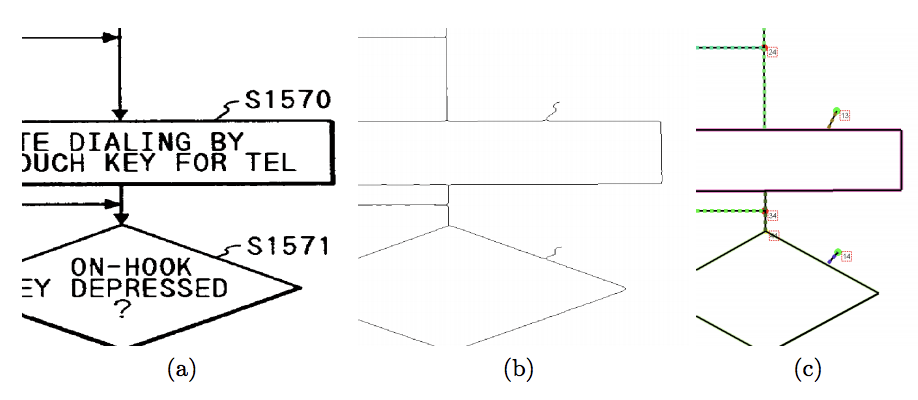
\includegraphics[scale=0.4]{RelatedWork.png}
  \caption{Process of flowchart retrieval. (a) Origin flowchart, (b) node detection and (c) retrieved flowchart.}
  \label{fig: RW1}
  \center
\end{figure}
    
    A recent patent reports a method for recognizing binary document such as table, pure text or flowchart~\cite{Ming2018}. The method first calculates the side of the image for top, bottom, left and right sides, then generates a boundary removal size for each side. After boundary removal for the four sides, it compares the side profiles to recognize the input document. Such method, however, cannot recognize the component within the flowchart.


\section{Methodology}
\subsection{Assumptions}
To make the objective achievable as course project, several assumptions are made and listed as below:

\begin{itemize}
    \item Each components in the hand-written flowchart should be closed graph.
    \item The arrows in the curve must be straight.
    \item The shape that can be recognized is restricted to rectangle, arrow, diamond and circle.
    \item No intersections among arrows.
\end{itemize}

\subsection{Pipeline}
Based on the assumptions above, the algorithm and pipeline is illustrated in Fig \ref{fig: Algorithm}. Details are explained in the following subsection.

\begin{figure*}
  \center
  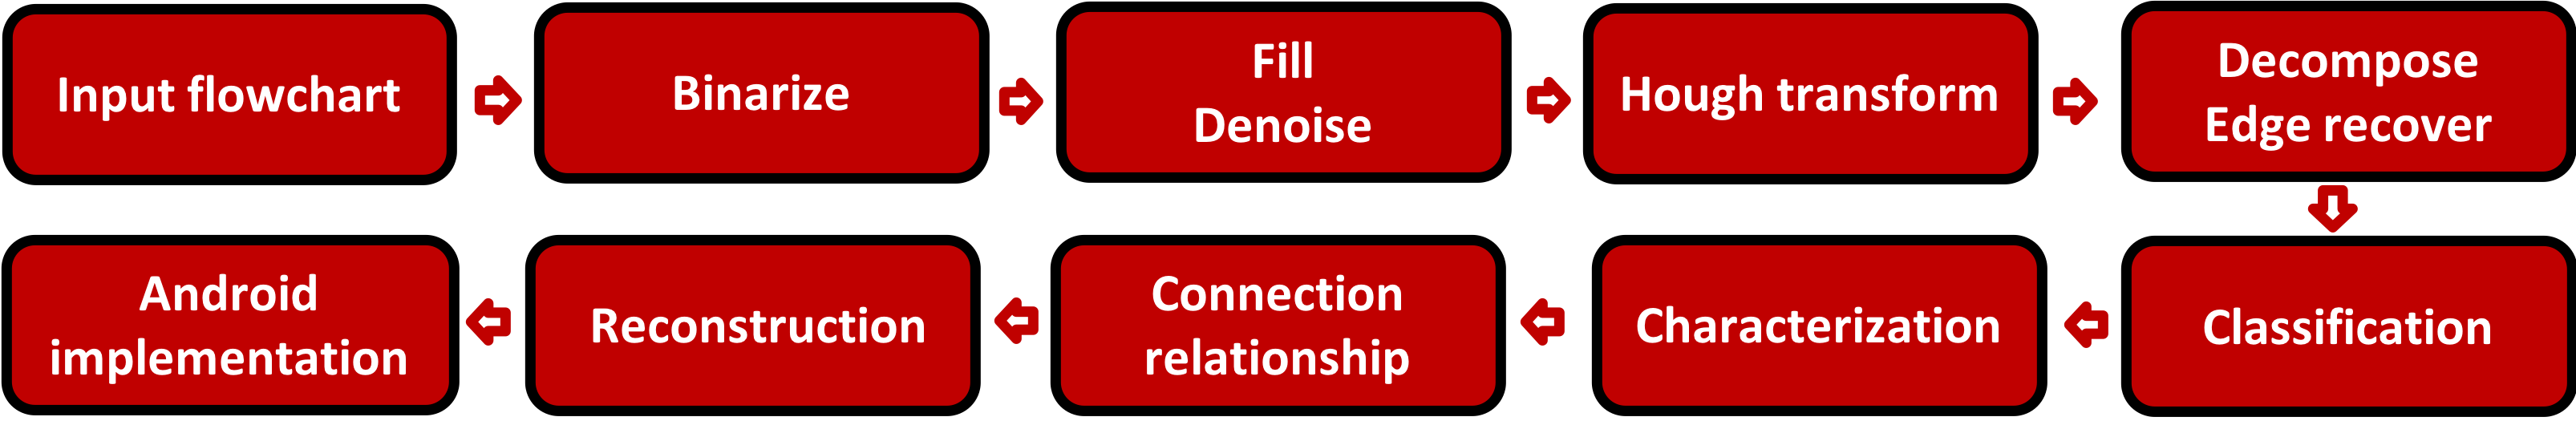
\includegraphics[scale=0.3]{Algorithm.png}
  \caption{Algorithm}
  \label{fig: Algorithm}
  \center
\end{figure*}


\subsubsection{Input Flowchart}
The input of our pipeline is an image in .jpg format. This image can be loaded from Android device's photo library or detected from Android camera view. In this step, the image is also adjusted to a fixed size. Usually, we re-size the image for accelerating the following processing steps, since an extremely large high resolution image can take prohibitively long time.
        
\subsubsection{Binarize}

The input image usually has three channels, RGB. The first step in our pipeline is to convert this RGB image to a gray-scale image, as shown in Fig~\ref{fig:rgb2gray}. After converting the image into gray-scale, we employ an Gaussian filter to remove the salt-and-pepper noise caused by camera. The improvements can be observed explicitly after an adaptive-threshold binarization operation. The filter size for this binarization is tuned carefully, because it is pretty sensitive to the change of contrast and luminance. Now, we have an image with black front-ground flow chart shapes and white background. The final operation in this step is a bit-wise inversion, to swap the front-ground and background colors. The results of binarization and bit-wise inversion are shown in Fig~\ref{fig:binarization} and Fig~\ref{fig:bitwise}, respectively.

\begin{figure}[!htbp]
    \centering
    \subfigure[RGB Image]
    {
        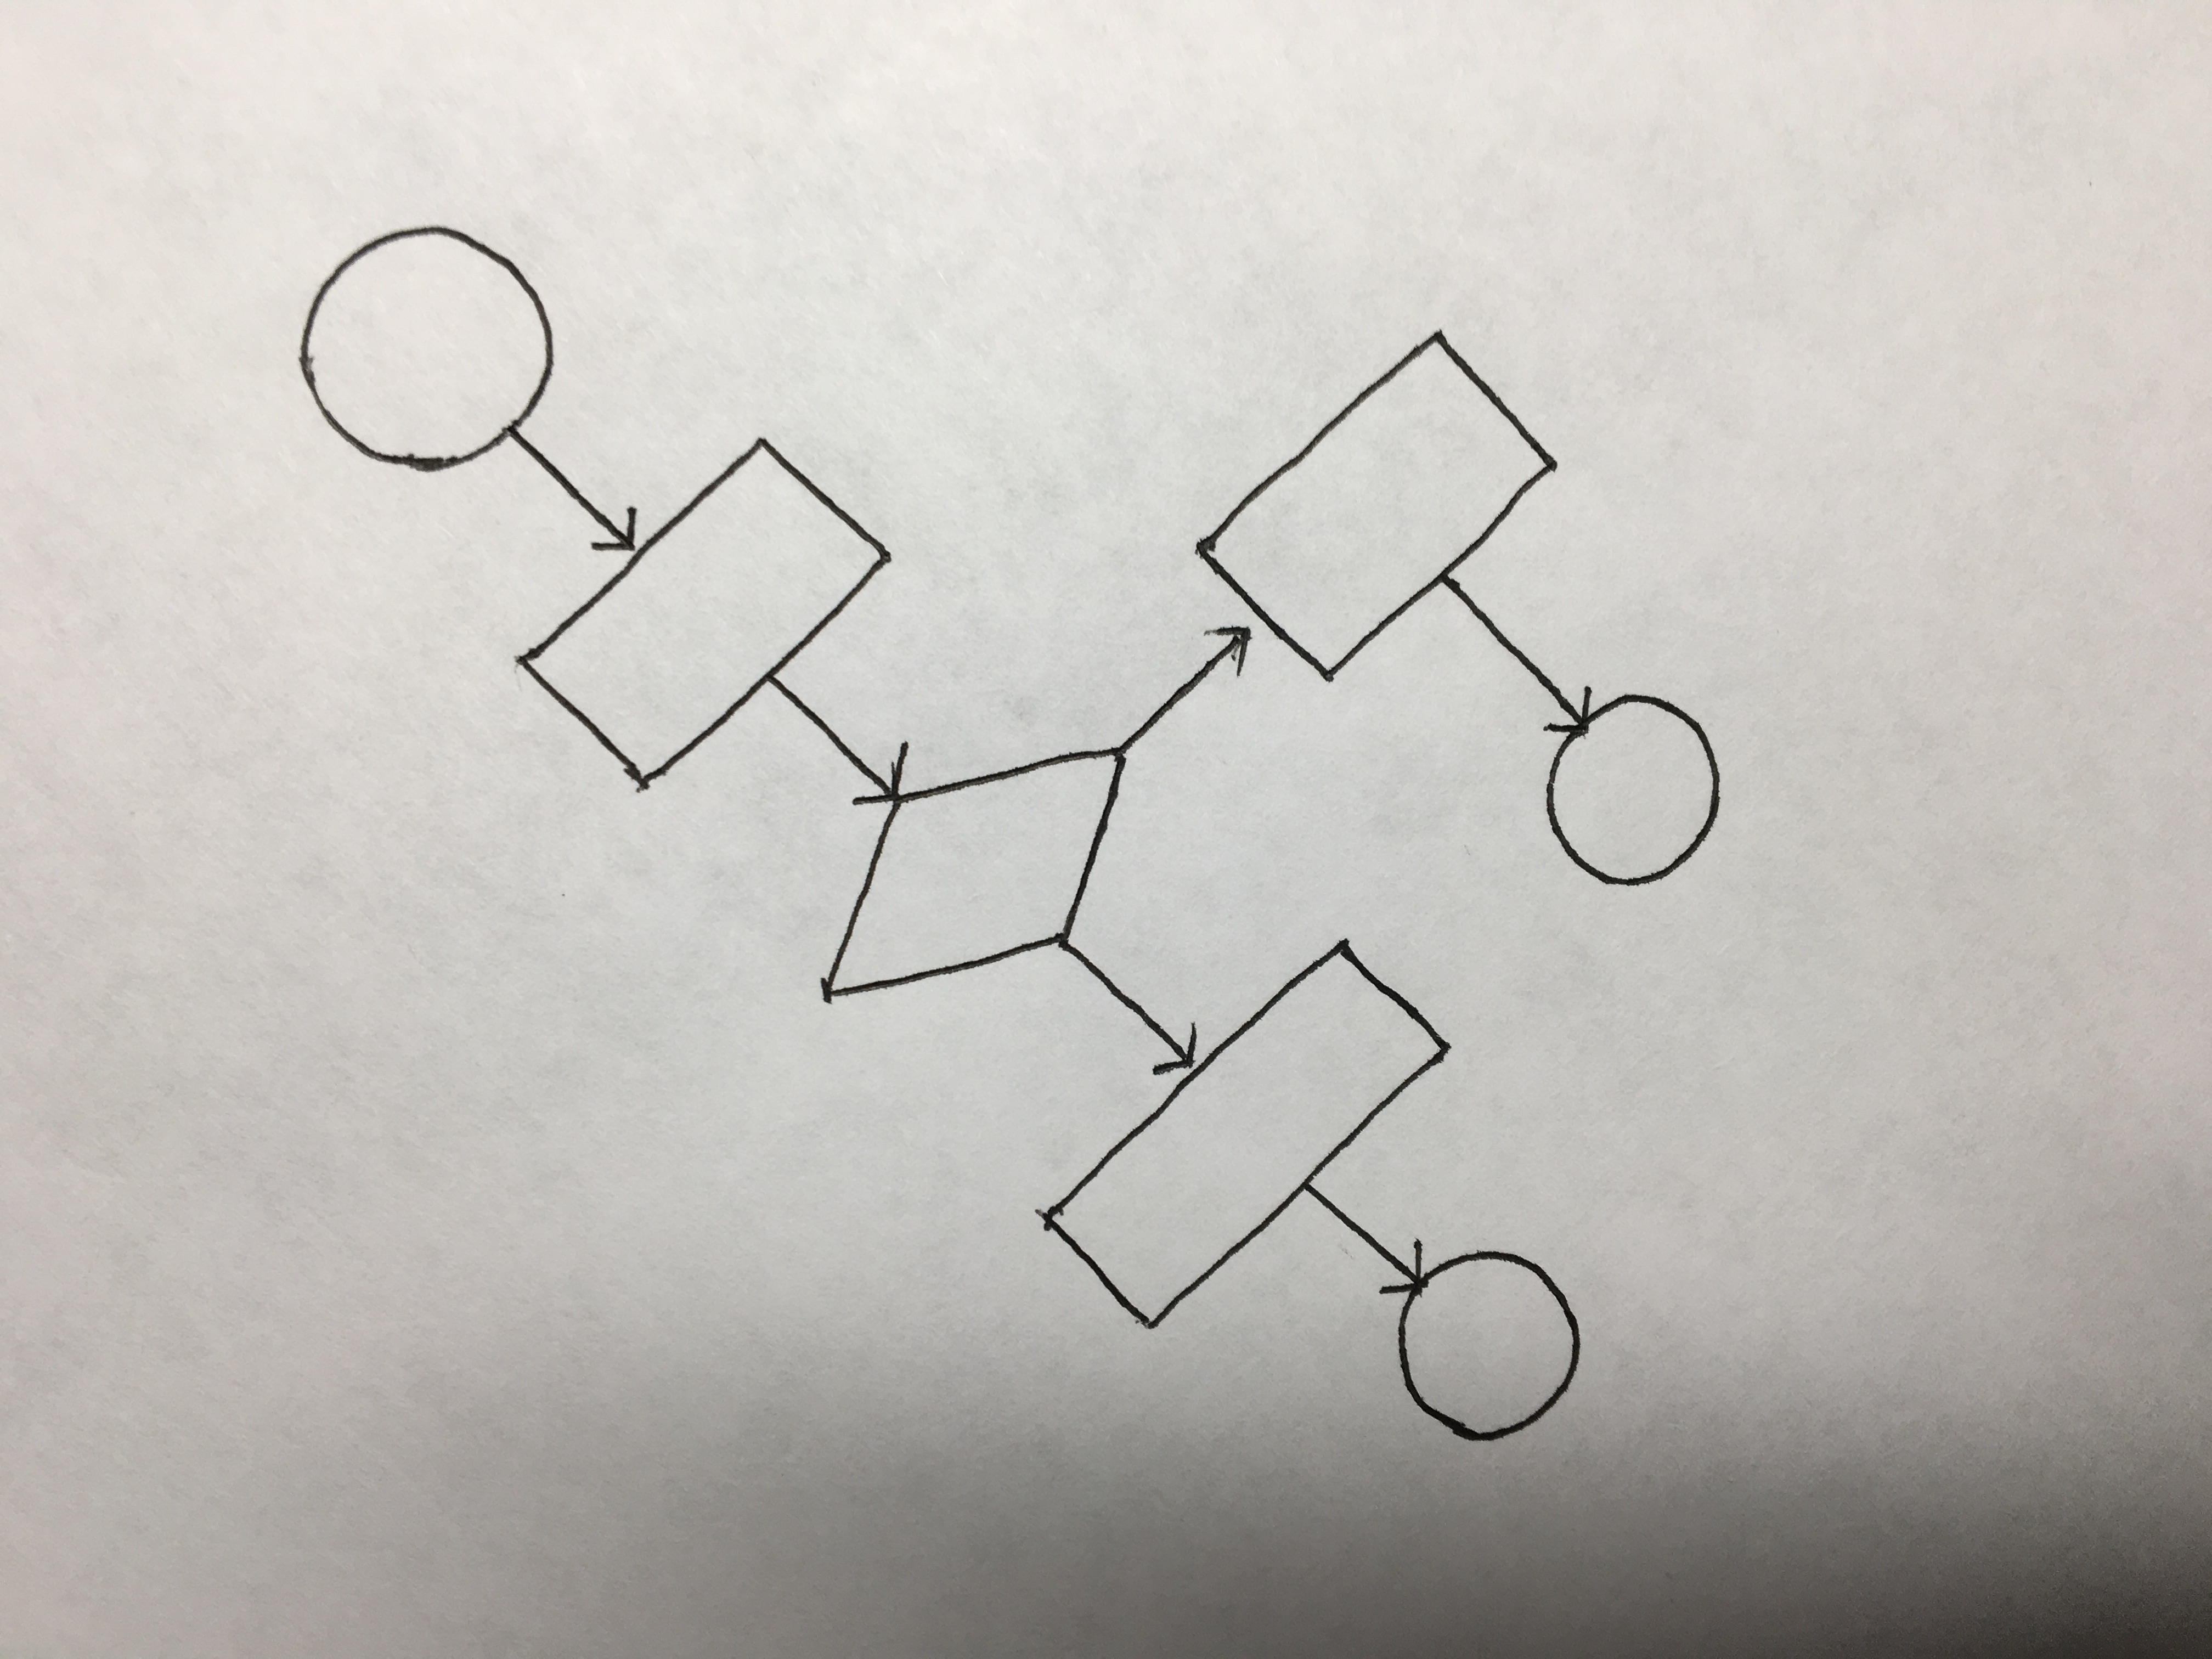
\includegraphics[angle=270, width=0.2\textwidth]{fig/you.JPG}
    }
    \subfigure[Gray-scale Image]
    {
        \includegraphics[angle=270, width=0.2\textwidth]{fig/gray.png}
    }
    \caption{Conversion from RGB to Gray-scale}
    \label{fig:rgb2gray}

\end{figure}


\begin{figure}[!htbp]
    \centering
    \subfigure[Gray-scale Image]
    {
        \includegraphics[angle=270, width=0.2\textwidth]{fig/gray.png}
    }
    \subfigure[Binary Image]
    {
        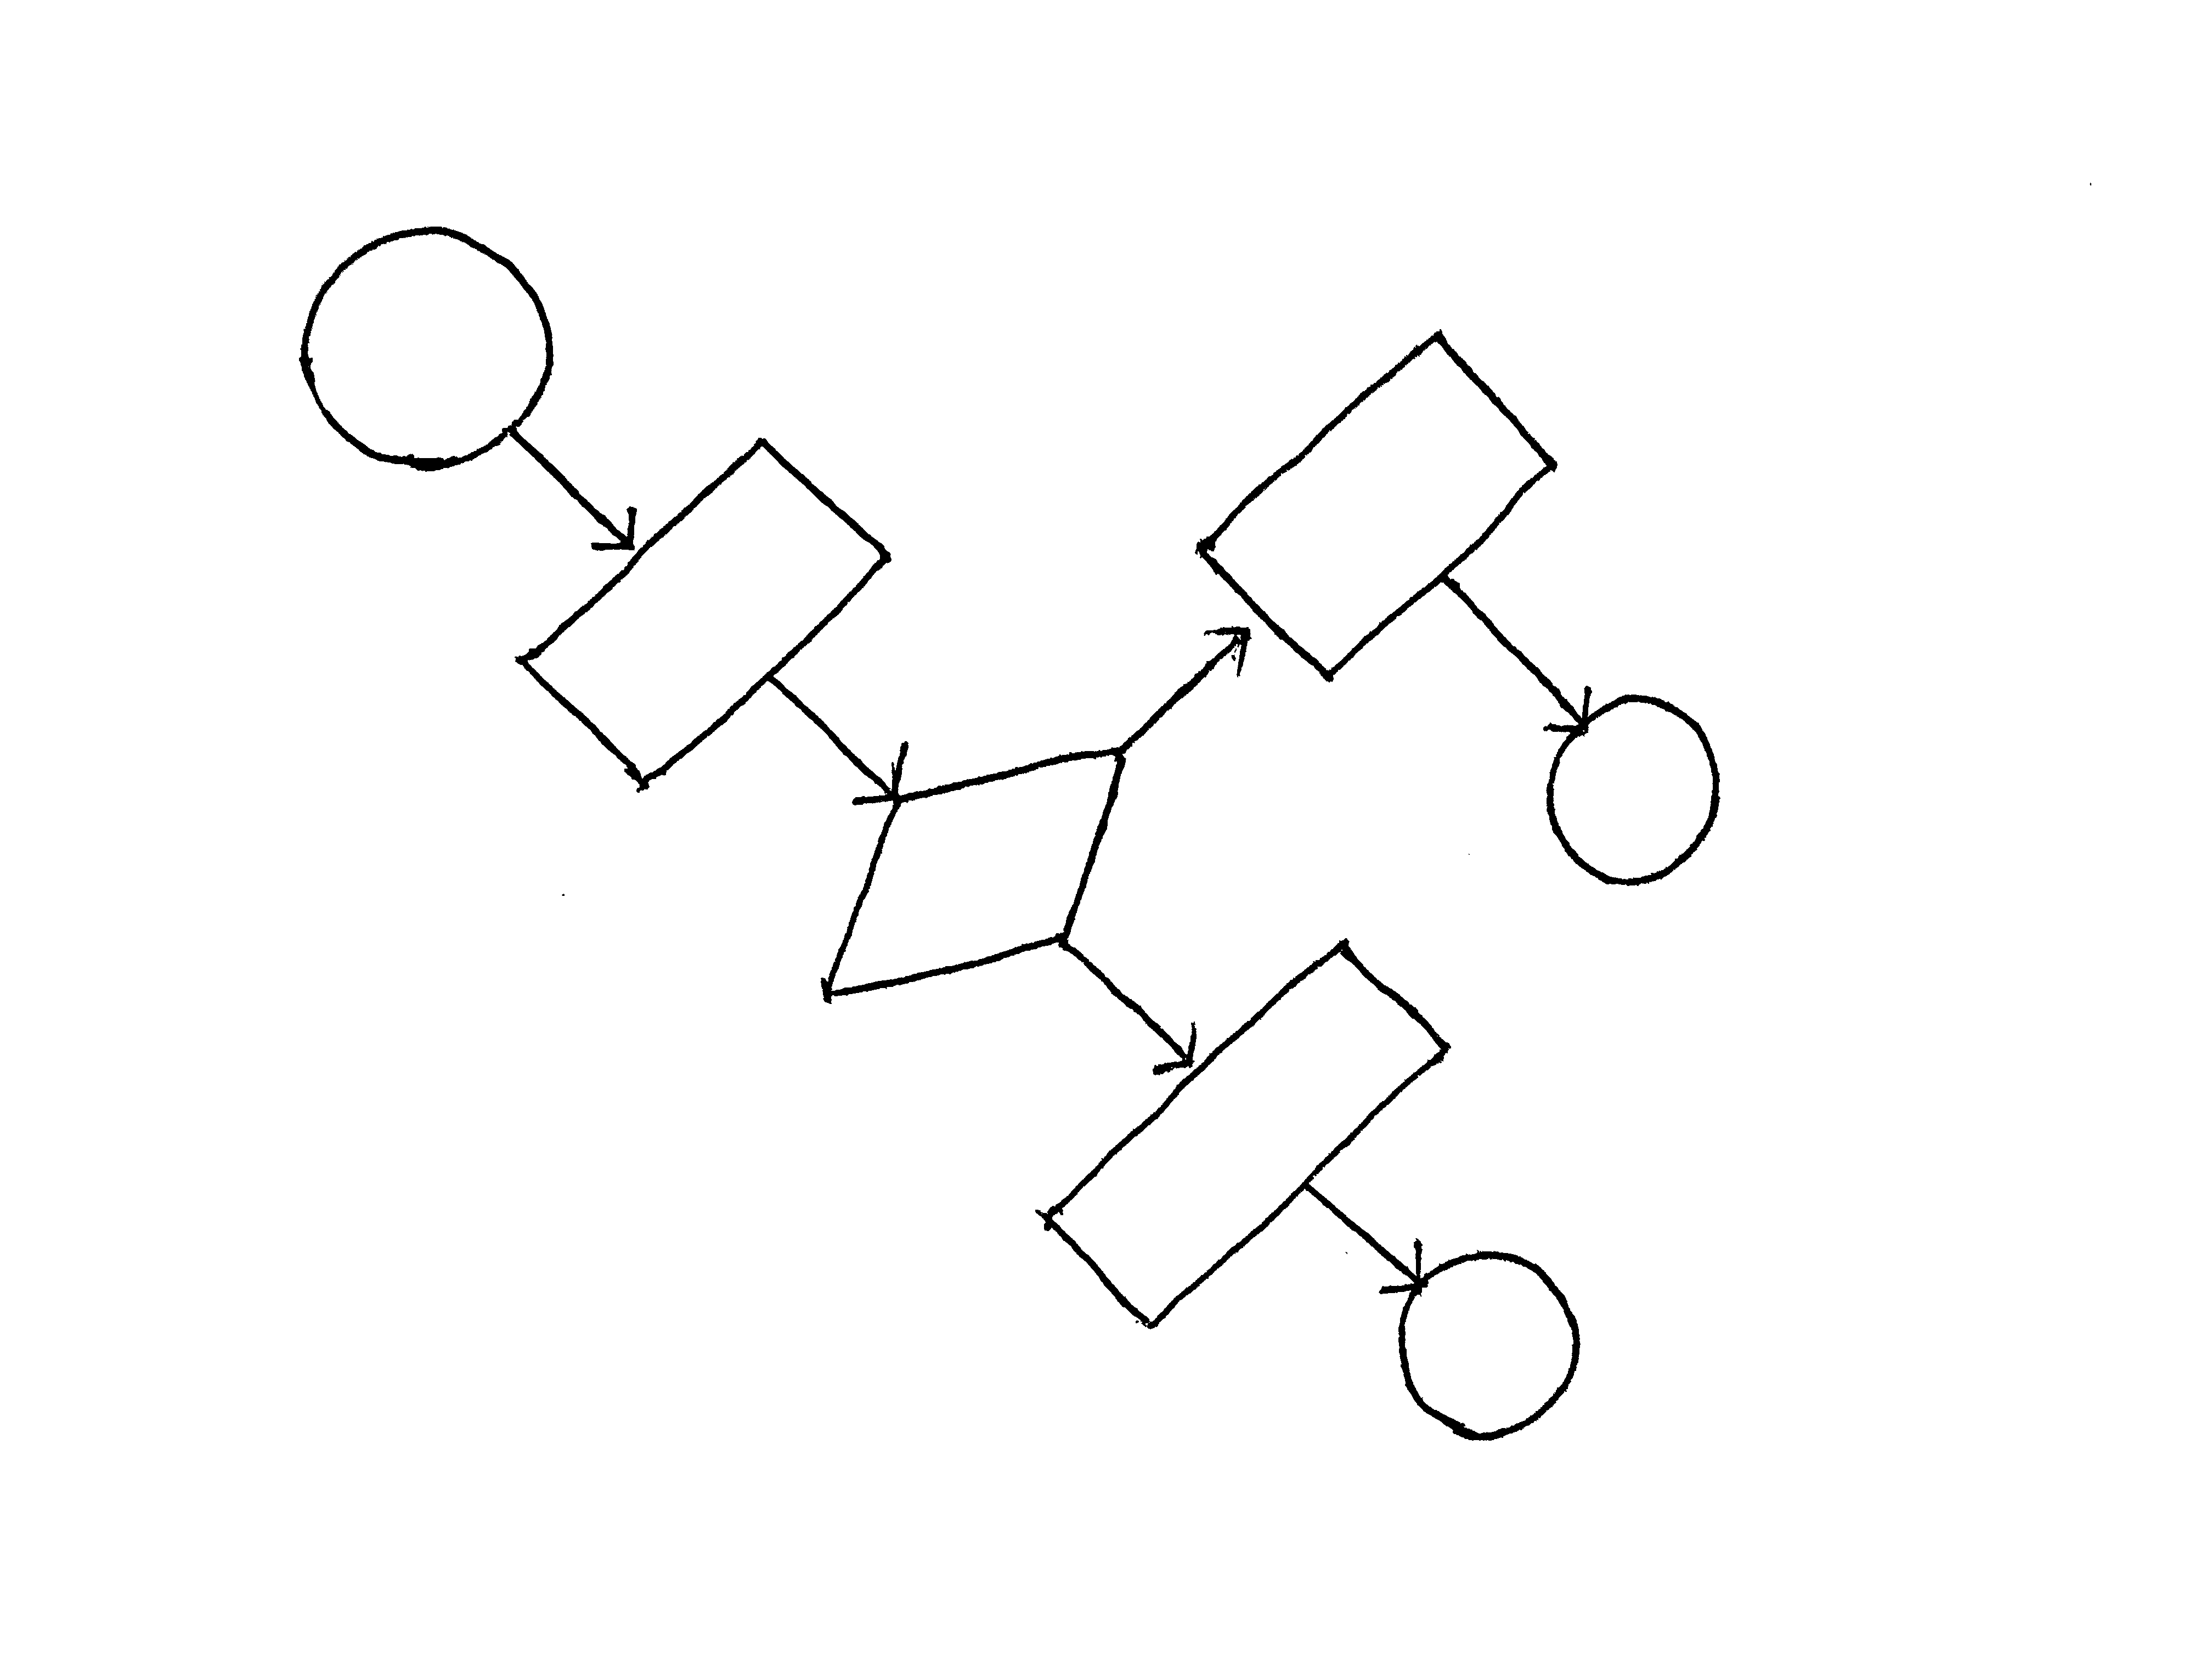
\includegraphics[angle=270, width=0.2\textwidth]{fig/bina.png}
    }
    \caption{Binarization}
    \label{fig:binarization}
\end{figure}


\begin{figure}[!htbp]
    \centering
    \subfigure[Binary Image]
    {
        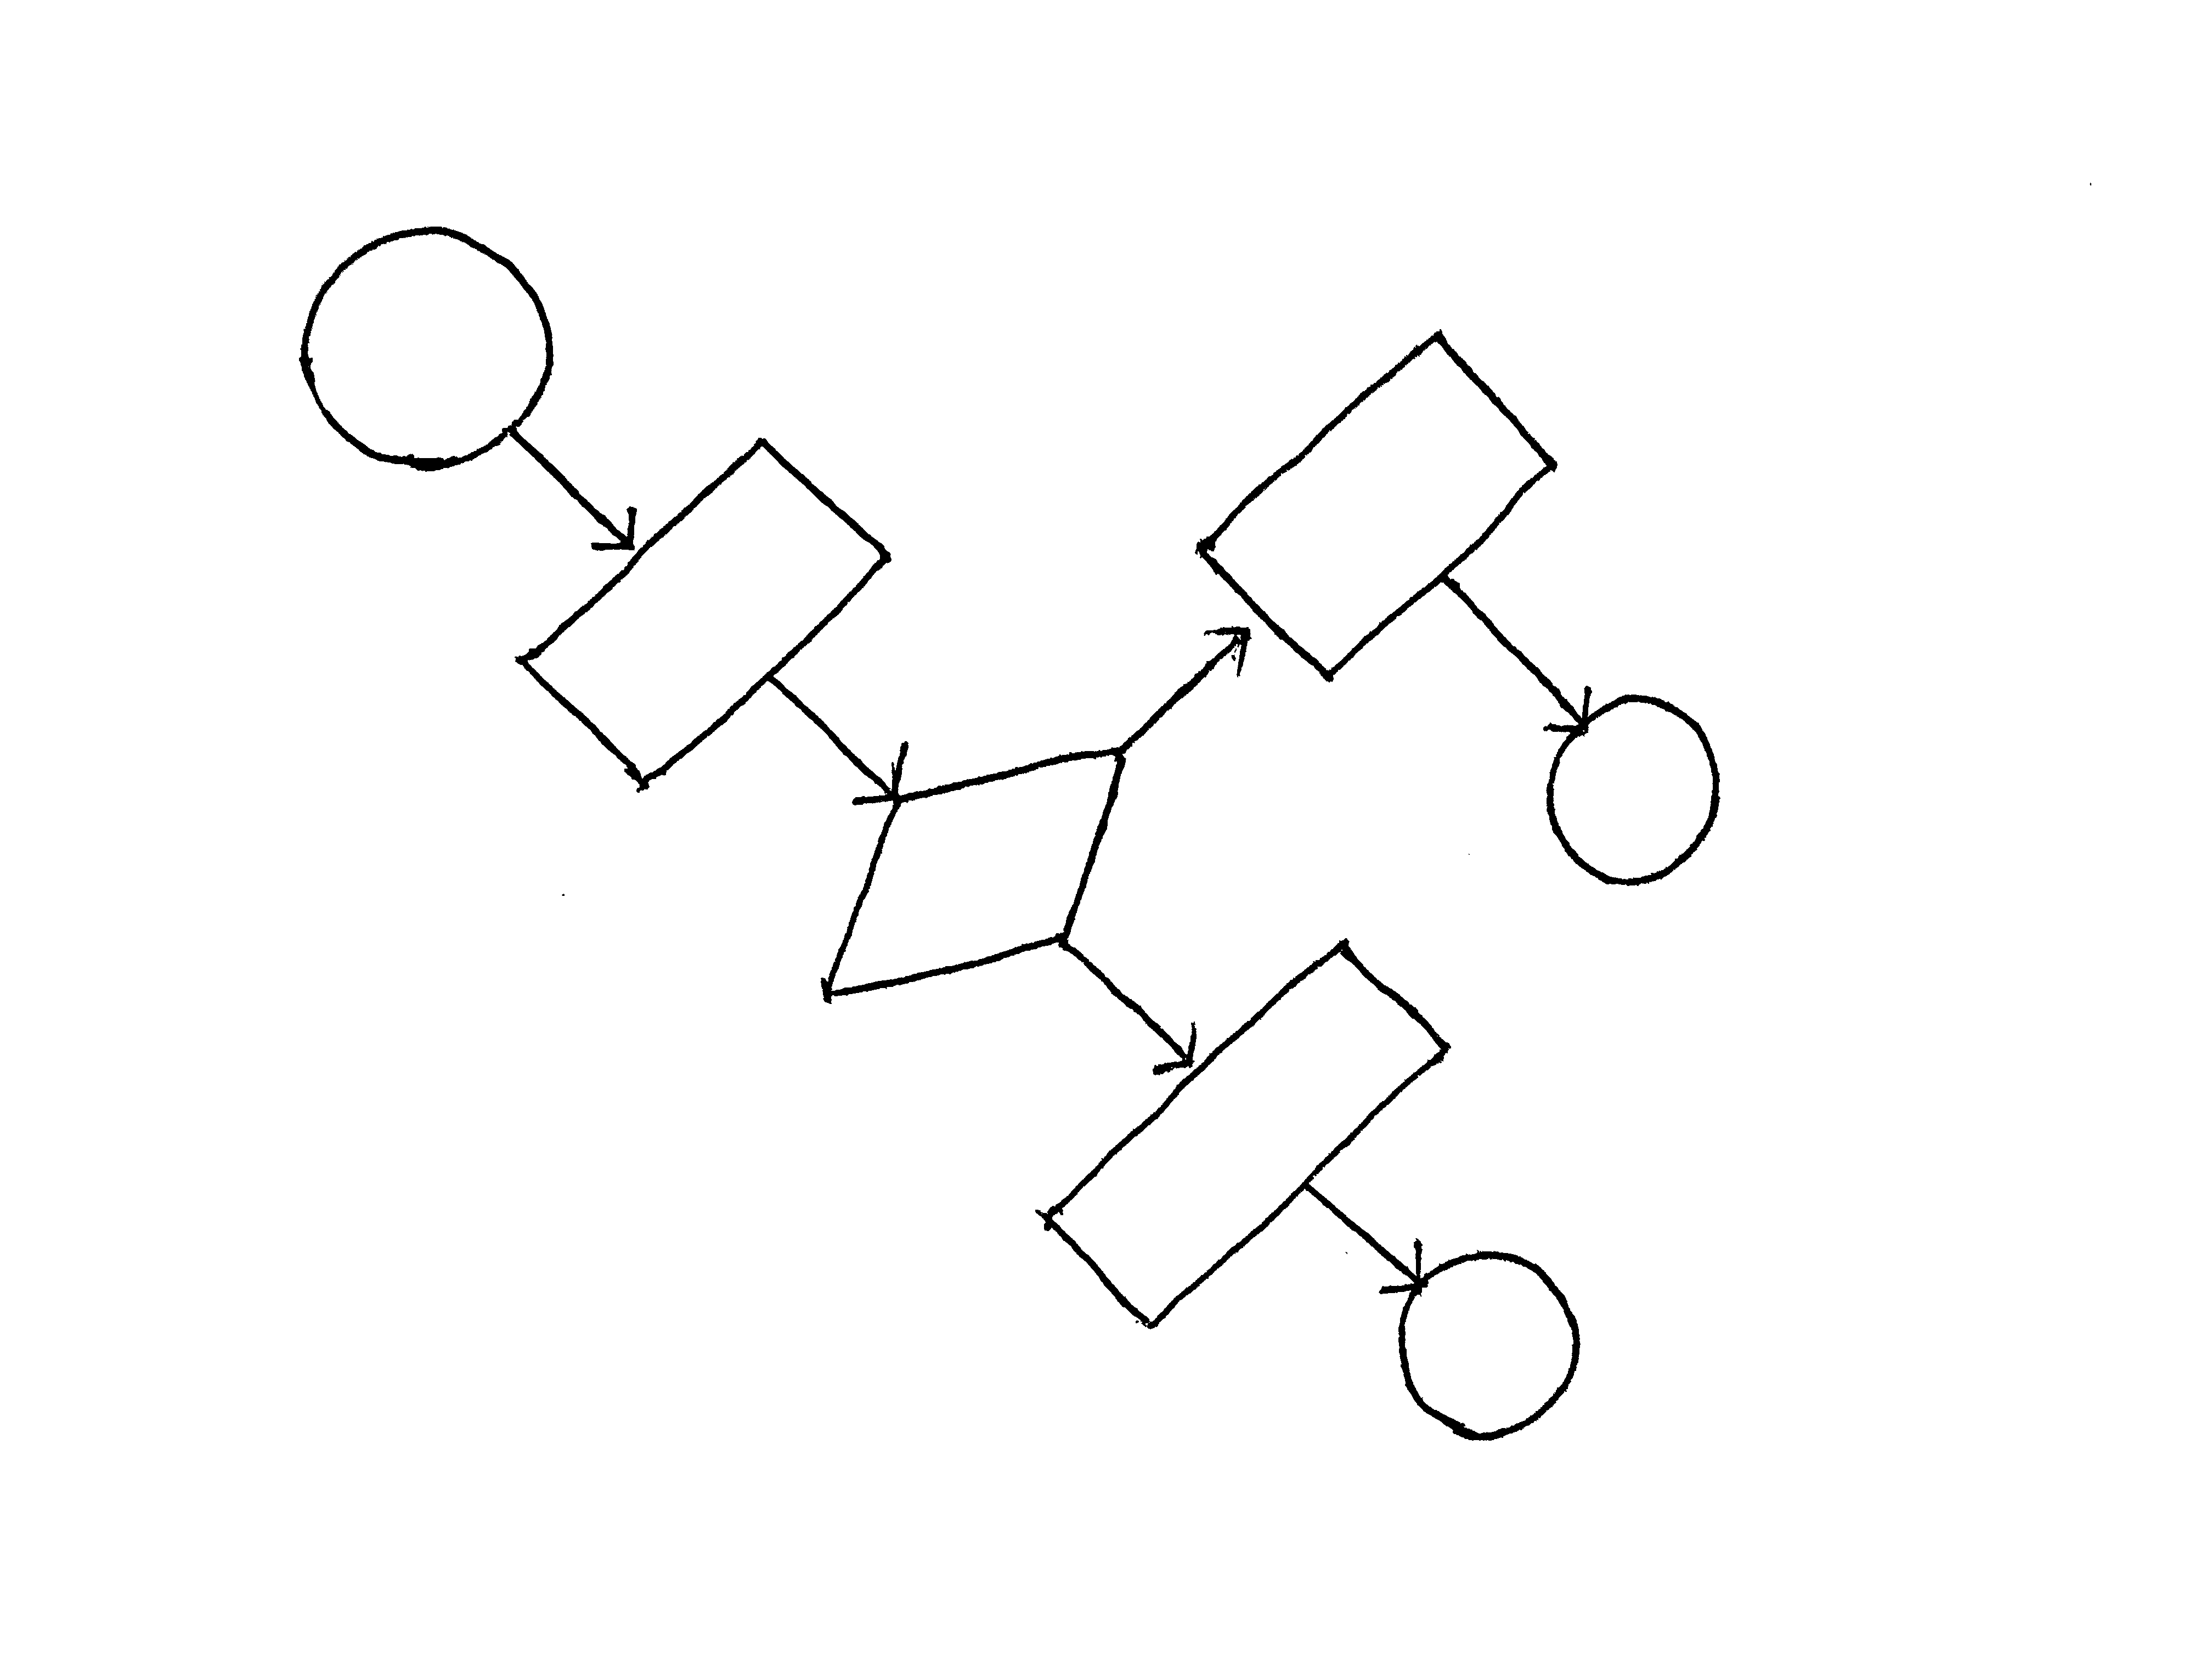
\includegraphics[angle=270, width=0.2\textwidth]{fig/bina.png}
    }
    \subfigure[Inverted Image]
    {
        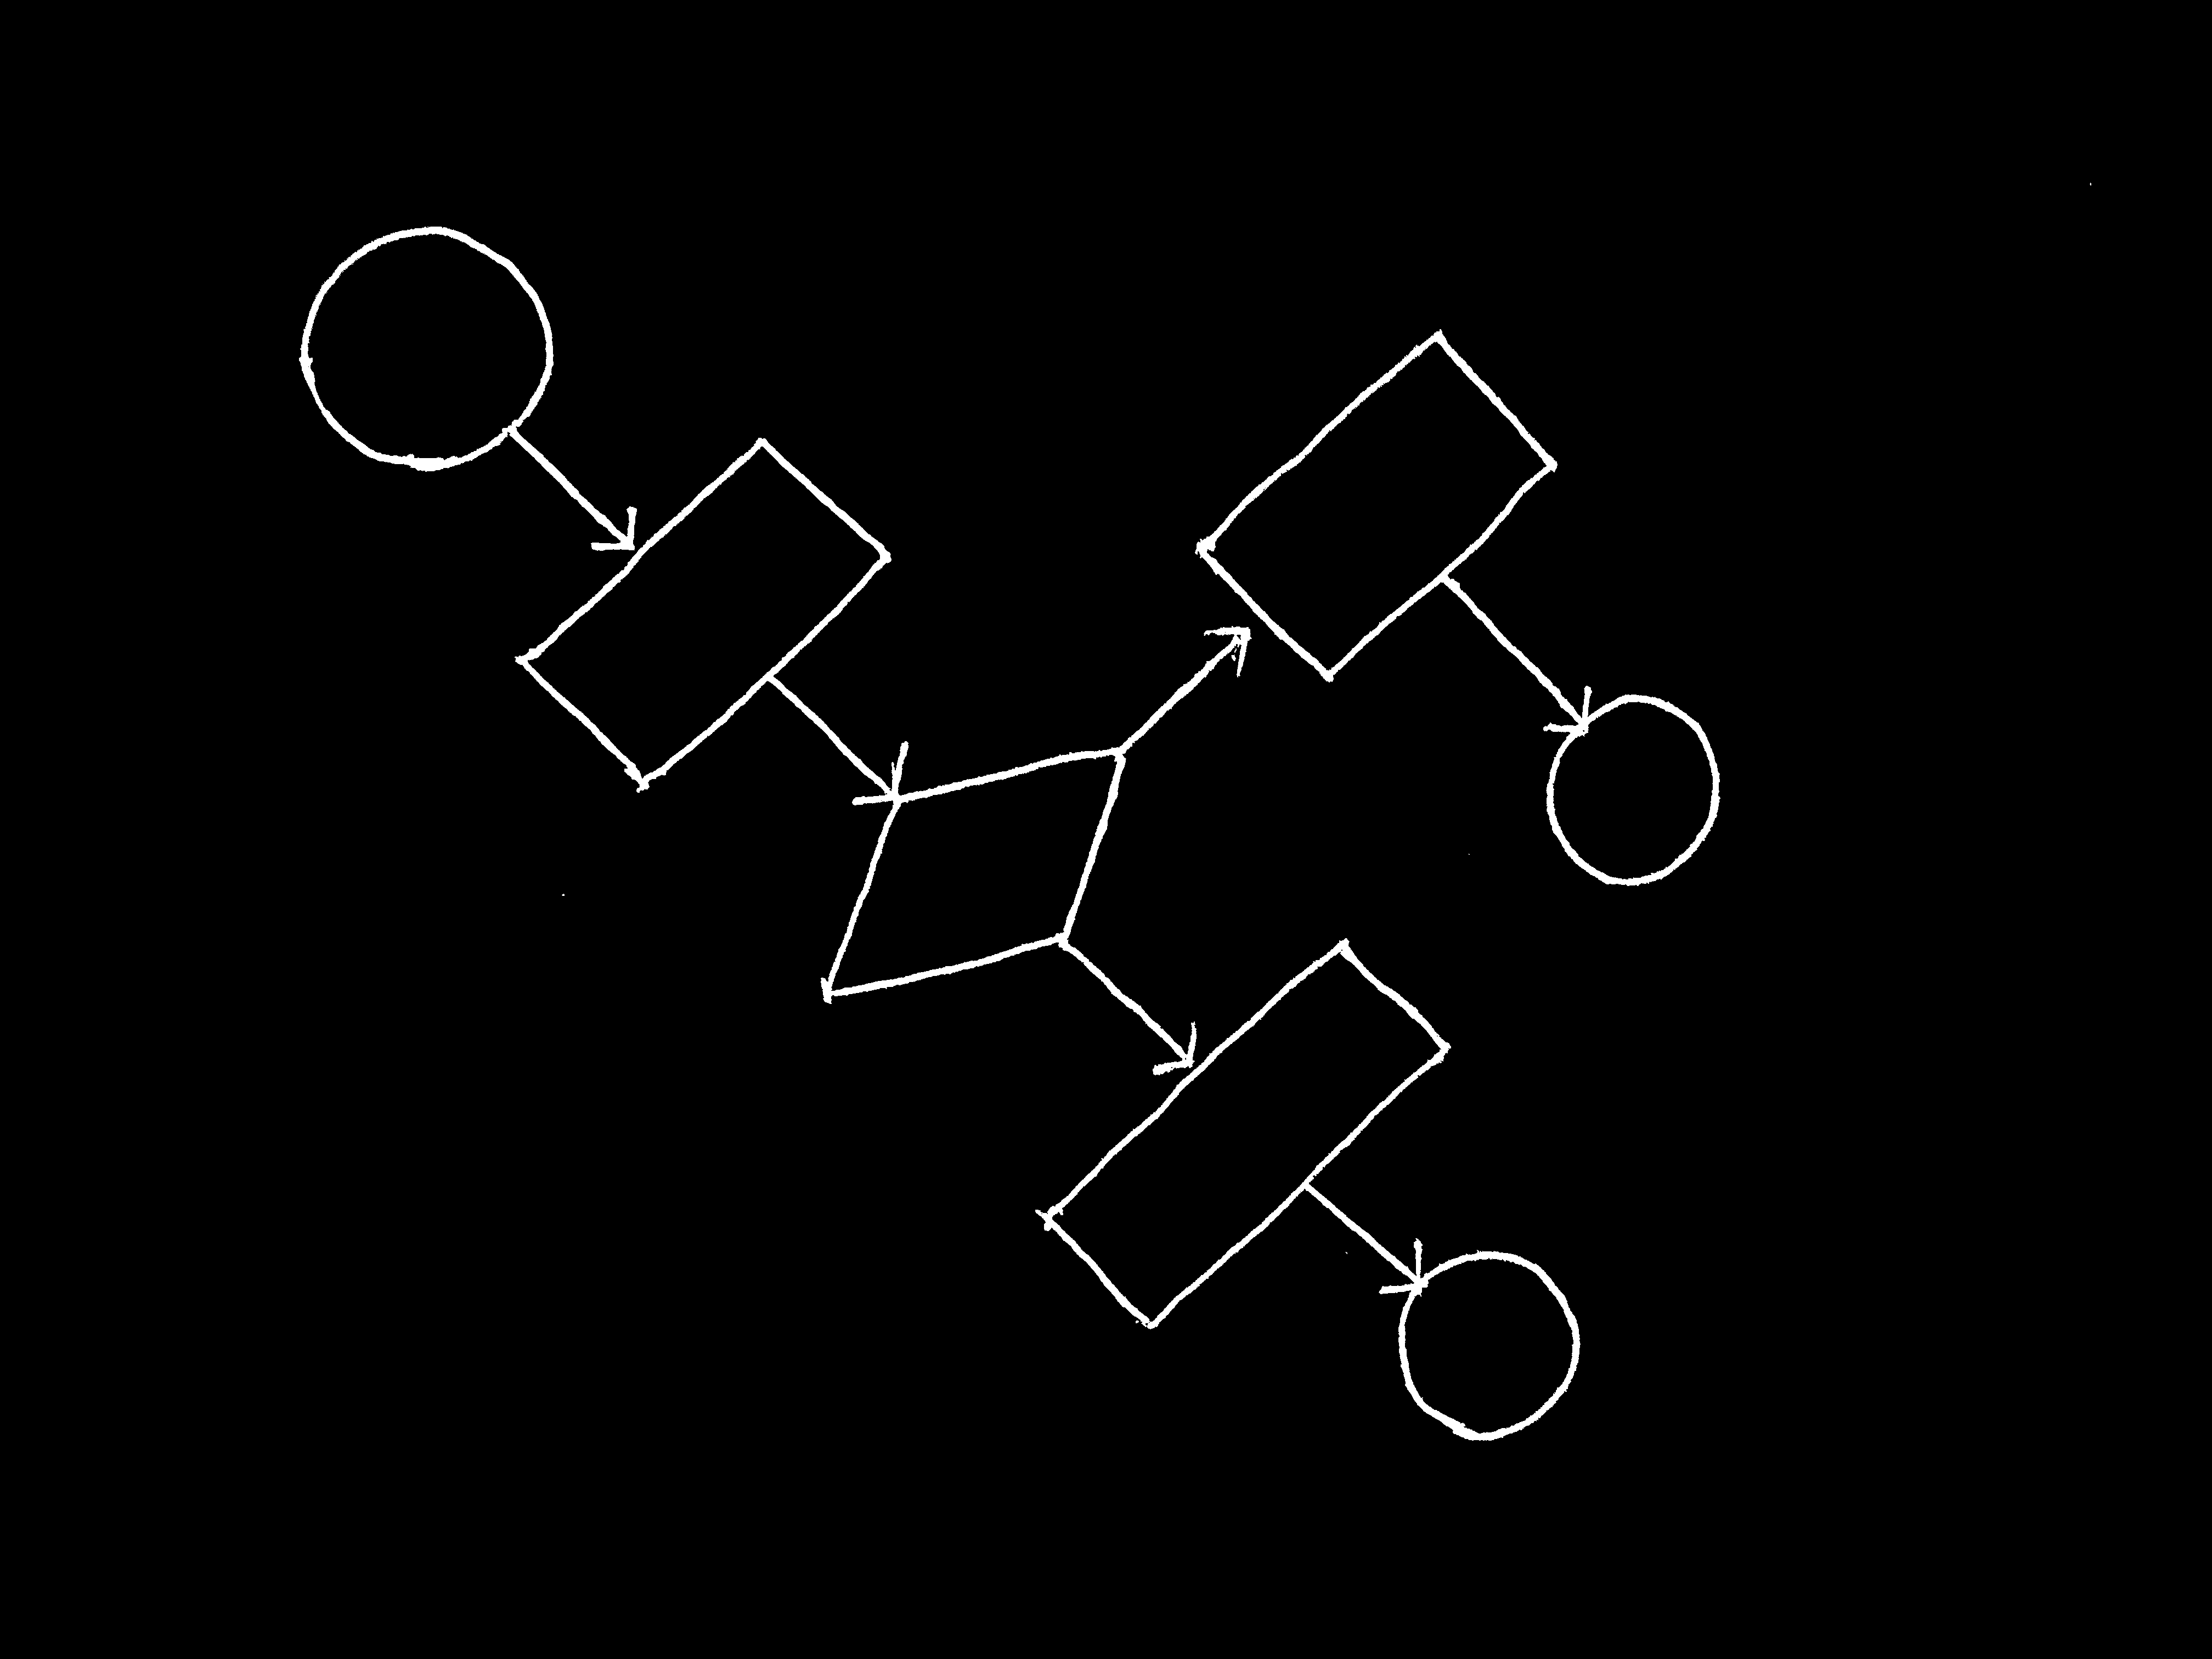
\includegraphics[angle=270, width=0.2\textwidth]{fig/invt.png}
    }
    \caption{Bit-wise Inversion}
    \label{fig:bitwise}
\end{figure}




\subsubsection{De-noising}
The de-noising operation is a little different from the one in the previous step. The "noise" in this step is the small areas that inappropriately generated by the binarization operation or caused by stains on the paper .Gaussian filter doesn't work again. Here, we remove all these small areas in another way. First, find all contours in the white fore-ground shapes. Second, fill black color into the contours with area smaller than the threshold we set. This procedure effectively eliminates all the irrelevant small areas and leaves the flow-chart in the background. The effect of Gaussian filter is shown in Fig~\ref{fig:gaussian} and that of small region removal is shown in Fig~\ref{fig:removal}.
and small region removal are shown in 

\begin{figure}[!htbp]
    \centering
    \subfigure[Before Gaussian Filter]
    {
        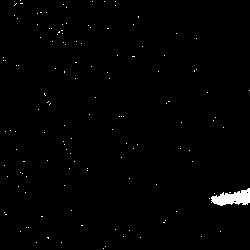
\includegraphics[angle=0, width=0.2\textwidth]{fig/noised.png}
    }
    \subfigure[After Gaussian Filter]
    {
        
\includegraphics[angle=0, width=0.2\textwidth]{fig/no_noise.png}
    }
    \caption{Gaussian Filtering}
    \label{fig:gaussian}
\end{figure}


\begin{figure}[!htbp]
    \centering
    \subfigure[Before Small Region Removal]
    {
        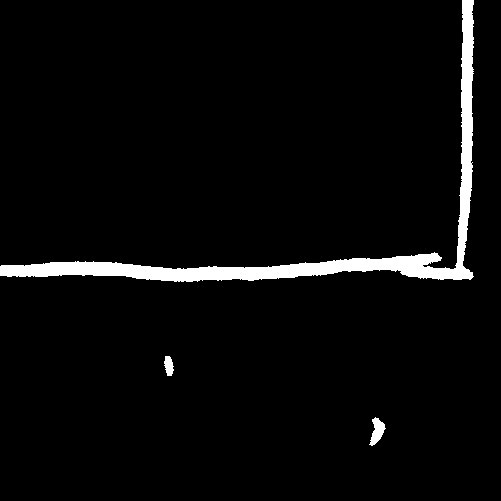
\includegraphics[angle=0, width=0.2\textwidth]{fig/beforeSmallRegionRemoval.png}
    }
    \subfigure[After Small Region Removal]
    {
        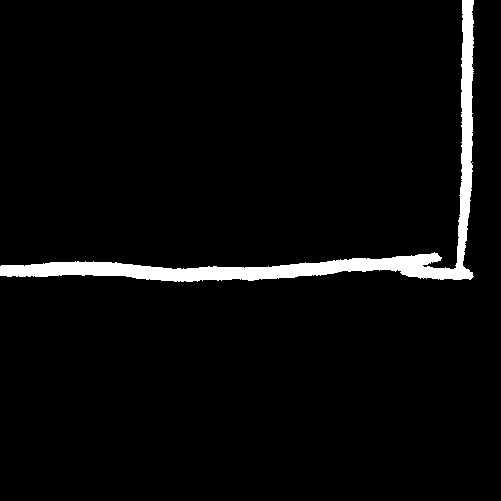
\includegraphics[angle=0, width=0.2\textwidth]{fig/afterSmallRegionRemoval.png}
    }
    \caption{Small Region Removal}
    \label{fig:removal}
\end{figure}

\subsubsection{Hough Transform and Rotation}
In this step, we want to make the flow chart to stay horizontally or vertically instead of tilted. This operation will be beneficial in the shape recognition and classification. The way to implement this is first to detect all edges in the image, as shown in Fig~\ref{fig:edgeDetect}. These edges will be analyzed by Hough transform to extract their angles. A histogram is generated then according to these angles. Among all the bins, the one with largest count is regarded as the primary angle. Thus, rotation is made based on this angle to reconstruct the correct direction for the flow chart. Here, we employ a two-step search to find the bin containing the primary angle. The first search is a coarse search with 180 degrees divided into 10 bins. the second search is a fine search with 18 degrees divided into 18 bins. In the example, we find the rotated angle is 45 degree clockwise, as shown in Fig~\ref{fig: histogram}. However, there is one more problem. The interface of rotation provided by OpenCV doesn't keep the whole image after rotation, instead it keeps the size of the original image, therefore, the corners of the image are cropped. Hence, we need to enlarge and shift the image before rotating it. This involves some calculation of the new width, new height as well as an expected shift. With of loss of generality, let's assume the four vertices of this rectangular image are $(0, 0), (x, 0), (0, y)$ and $(x, y)$. The clock-wise coordinate rotation formula is
$$
\left( \begin{array}{cc}
x^\prime \\
y^\prime
\end{array} \right)
=
\left( \begin{array}{cc}
\cos\theta & \sin\theta \\
-\sin\theta & \cos\theta
\end{array} \right)
%
\left( \begin{array}{cc}
x \\
y
\end{array} \right)
$$
After a rotation of angle $\theta$, we can obtain the four rotated vertices. They are respectively $(0, 0), (x*\cos\theta, -x*\sin\theta), (y*\sin\theta, y*\cos\theta)$ and $ (x*\cos\theta+y*\sin\theta, -x*\sin\theta+y*\cos\theta)$.
Now, we can clearly know that if we have a clockwise rotation ($\theta$ is positive), the new width of the rotated image is $x * \cos\theta + y * \sin\theta$, the new height is $y * \cos\theta + x * \sin\theta$ and the shift is $x * \sin\theta$ along $y$-axis. If the rotation is counter-clockwise ($\theta$ is negative), the new width of the rotated image is $x * \cos\theta - y * \sin\theta$, the new height is $-x * \sin\theta + y * \cos\theta$ and the shift is $-y * \sin\theta$ along $x$-axis.
The effect of shift and rotation is shown in Fig~\ref{fig:rotation}.


\begin{figure}[!htbp]
    \centering
    \subfigure[Binary Image]
    {
        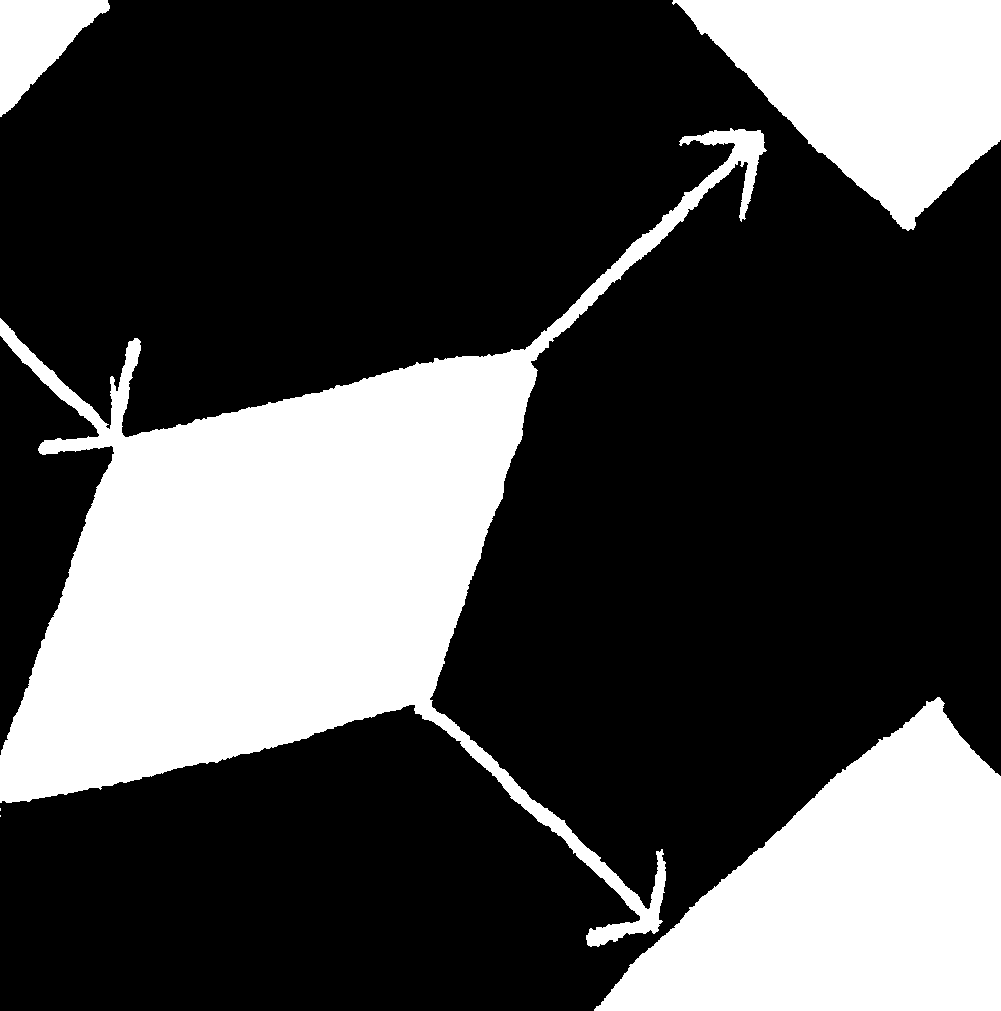
\includegraphics[angle=270, width=0.2\textwidth]{fig/orig.png}
    }
    \subfigure[Detected Edges]
    {
        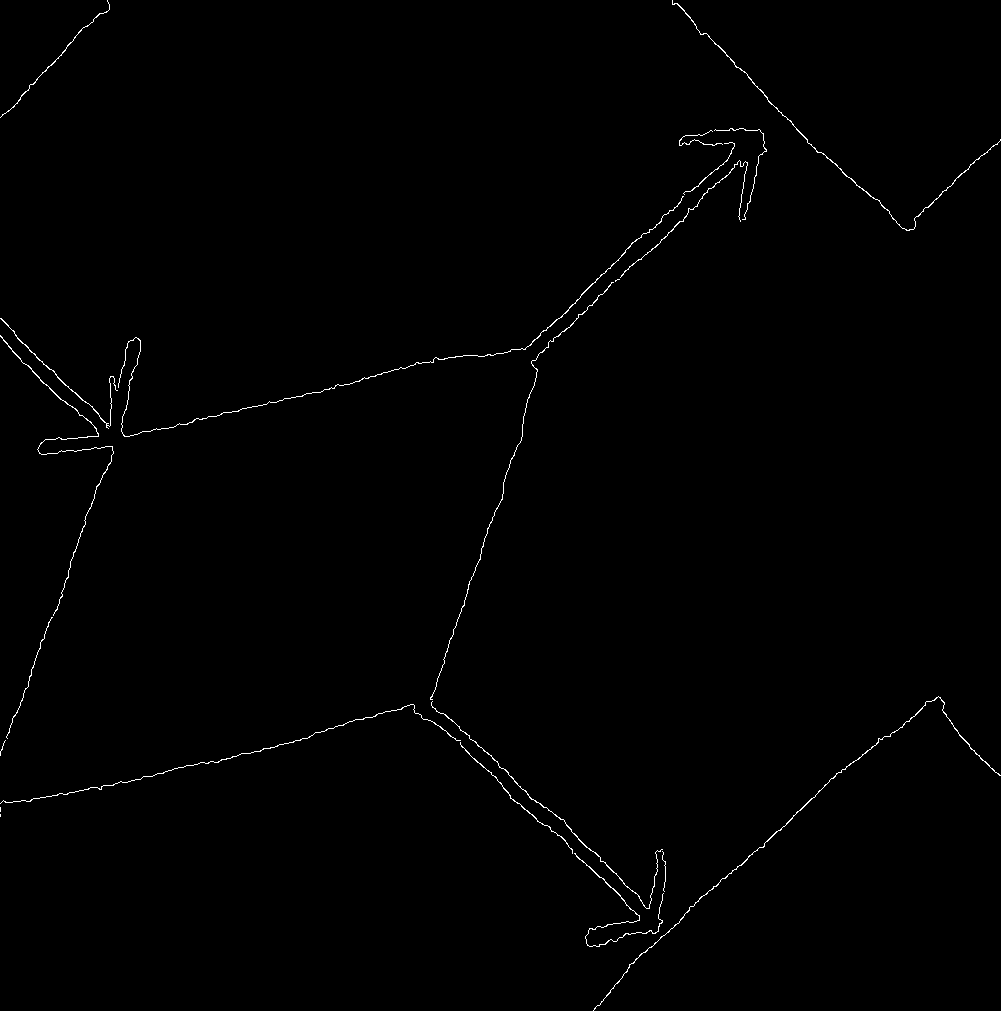
\includegraphics[angle=270, width=0.2\textwidth]{fig/edge.png}
    }
    \caption{Edge Detection}
    \label{fig:edgeDetect}
\end{figure}

\begin{figure}[!htbp]
\begin{center}
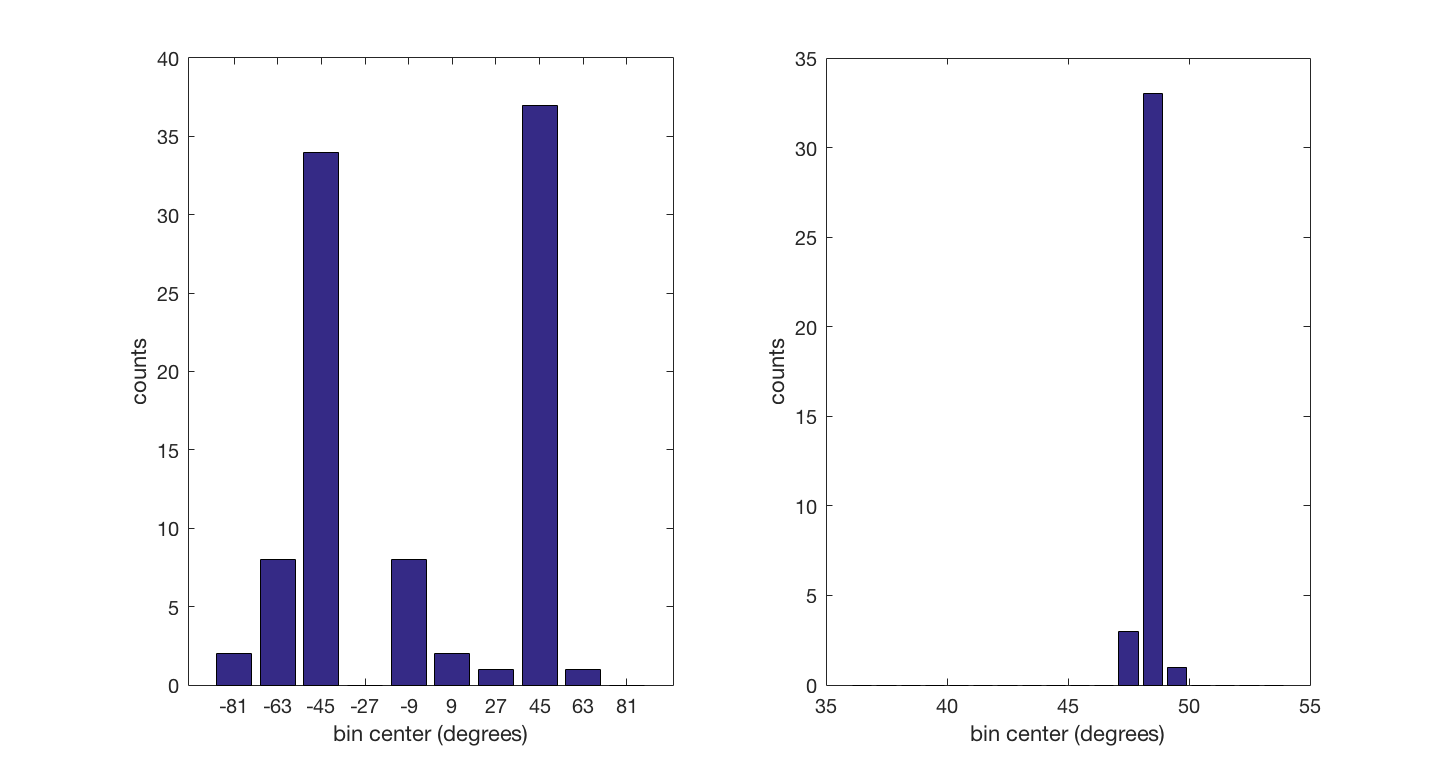
\includegraphics[width=0.48\textwidth]{fig/histogram.png}
\caption{Histogram of Rotated Degrees}
\label{fig: histogram}
\end{center}
\end{figure}

\begin{figure}[!htbp]
    \centering
    \subfigure[Binary Image]
    {
        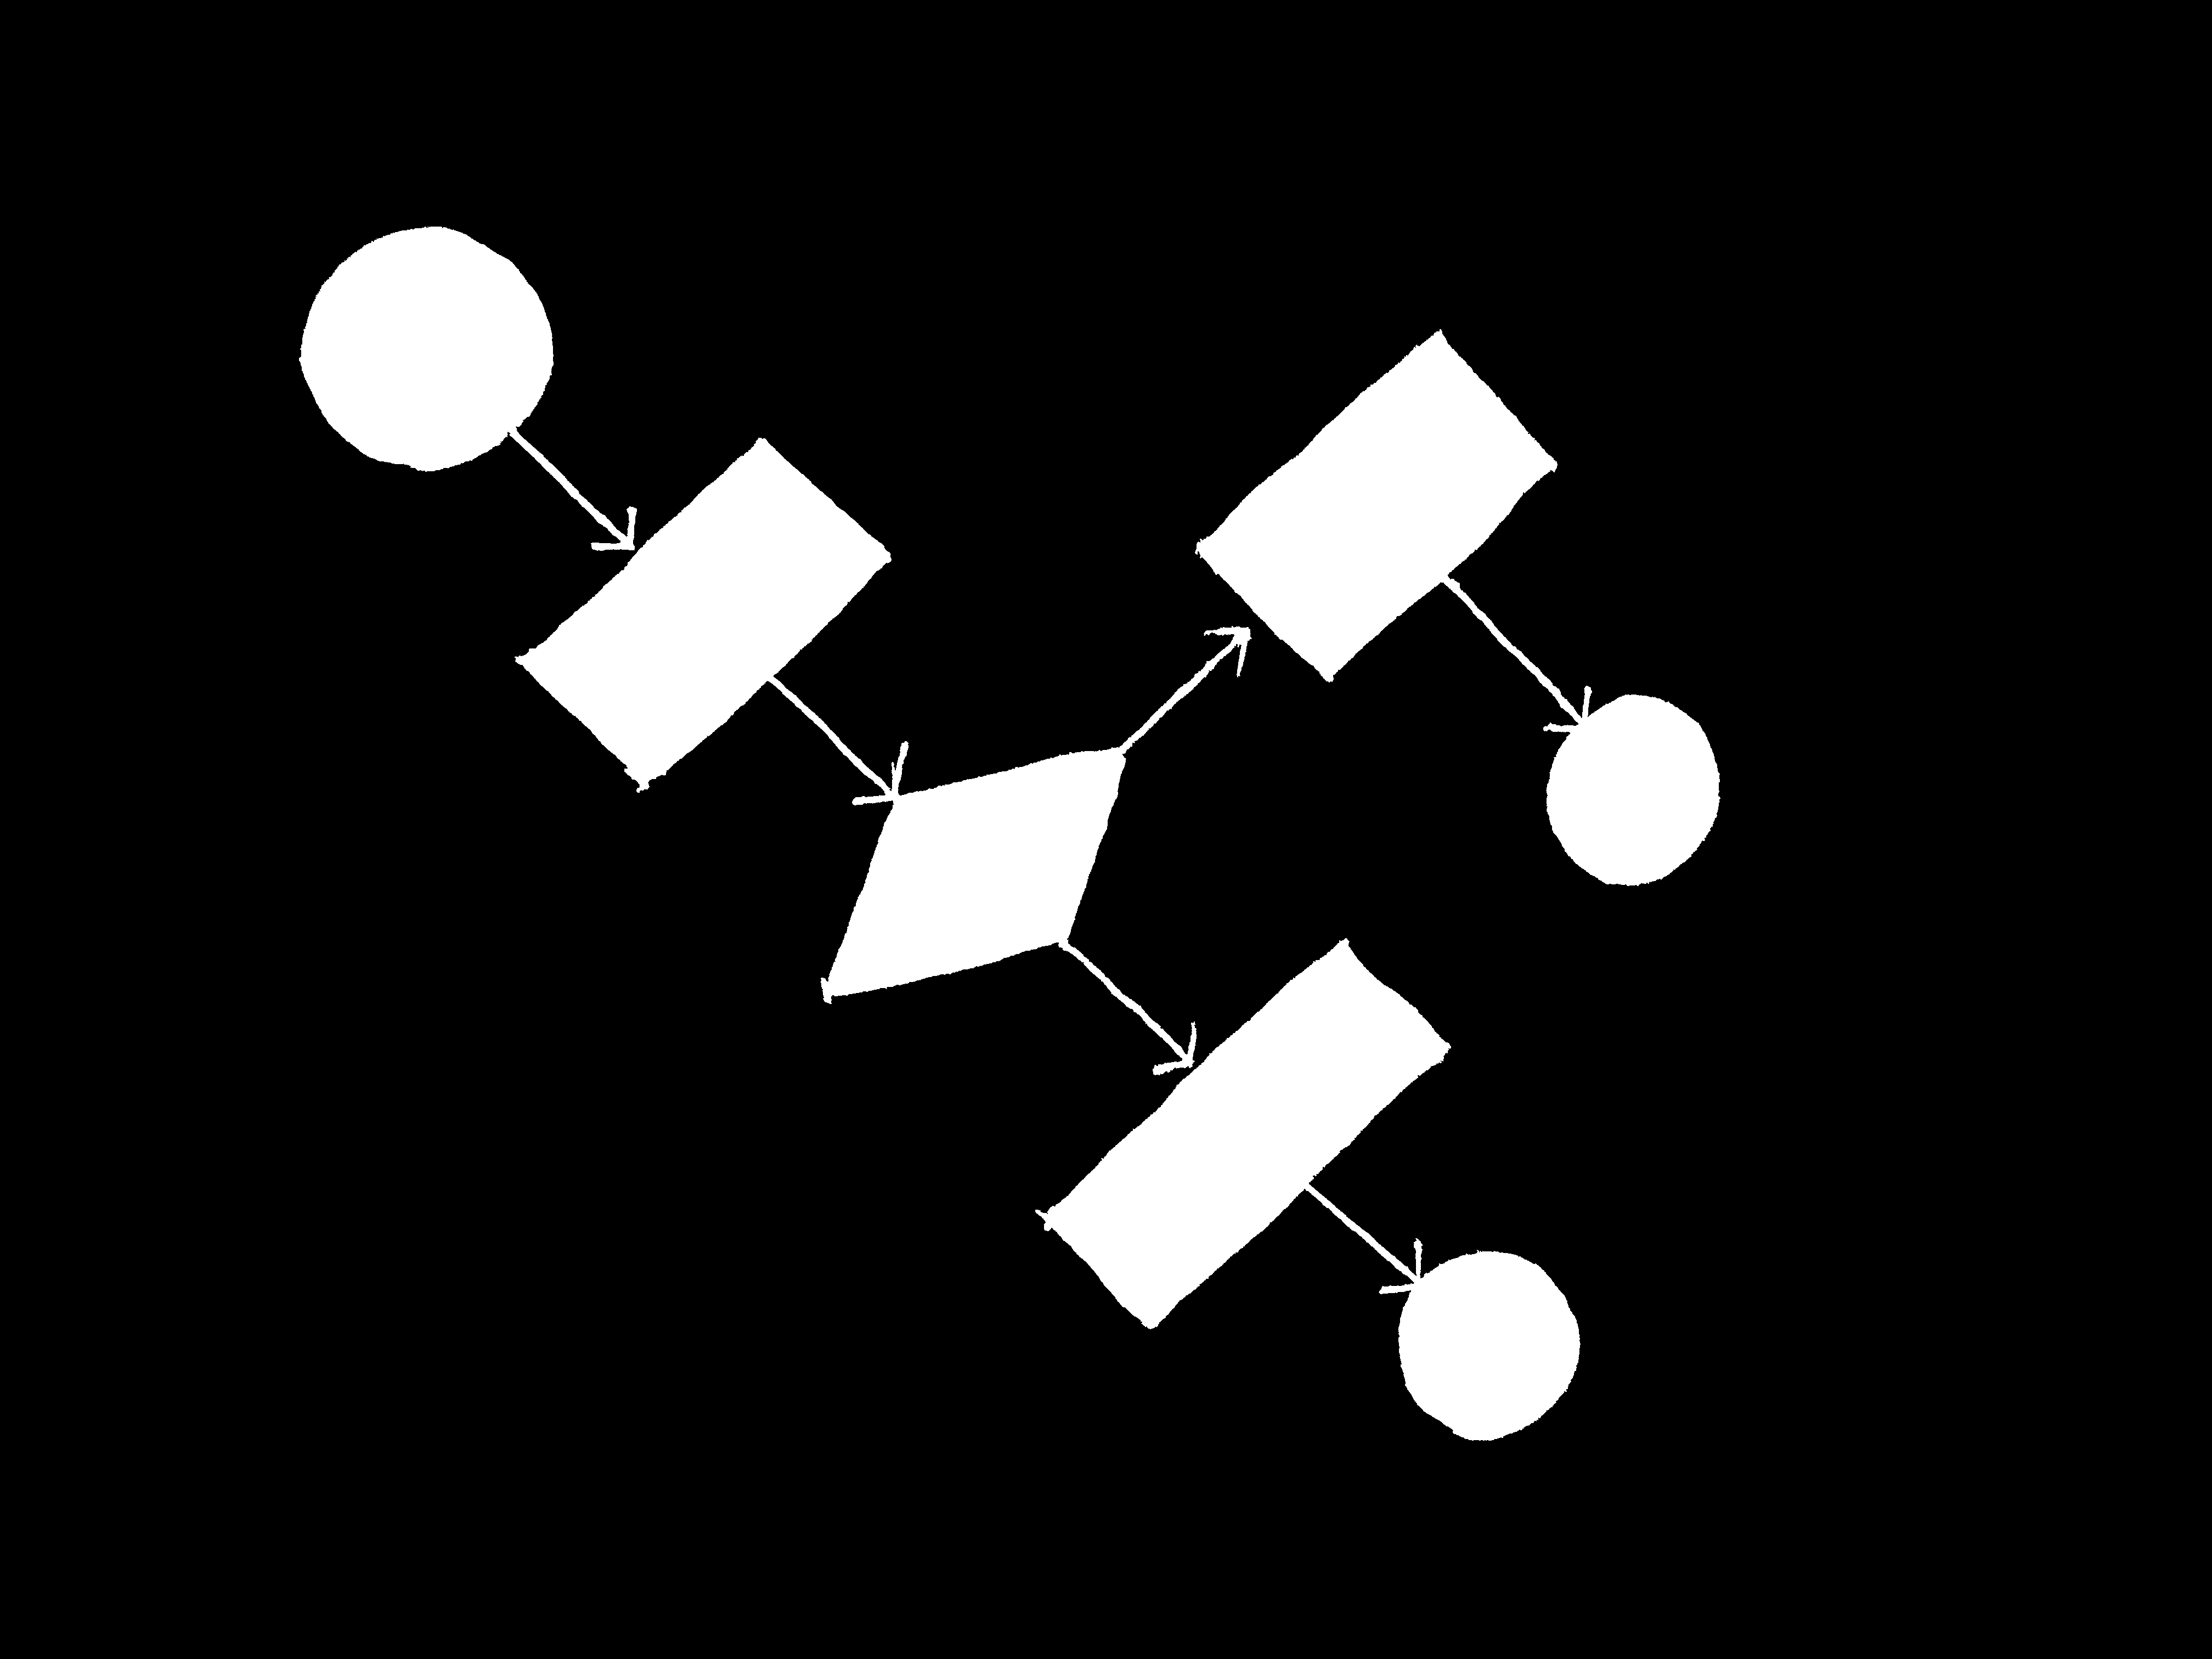
\includegraphics[height=2.8cm, angle=270]{fig/denoise.png}
    }
    \subfigure[After Shift and Rotation]
    {
        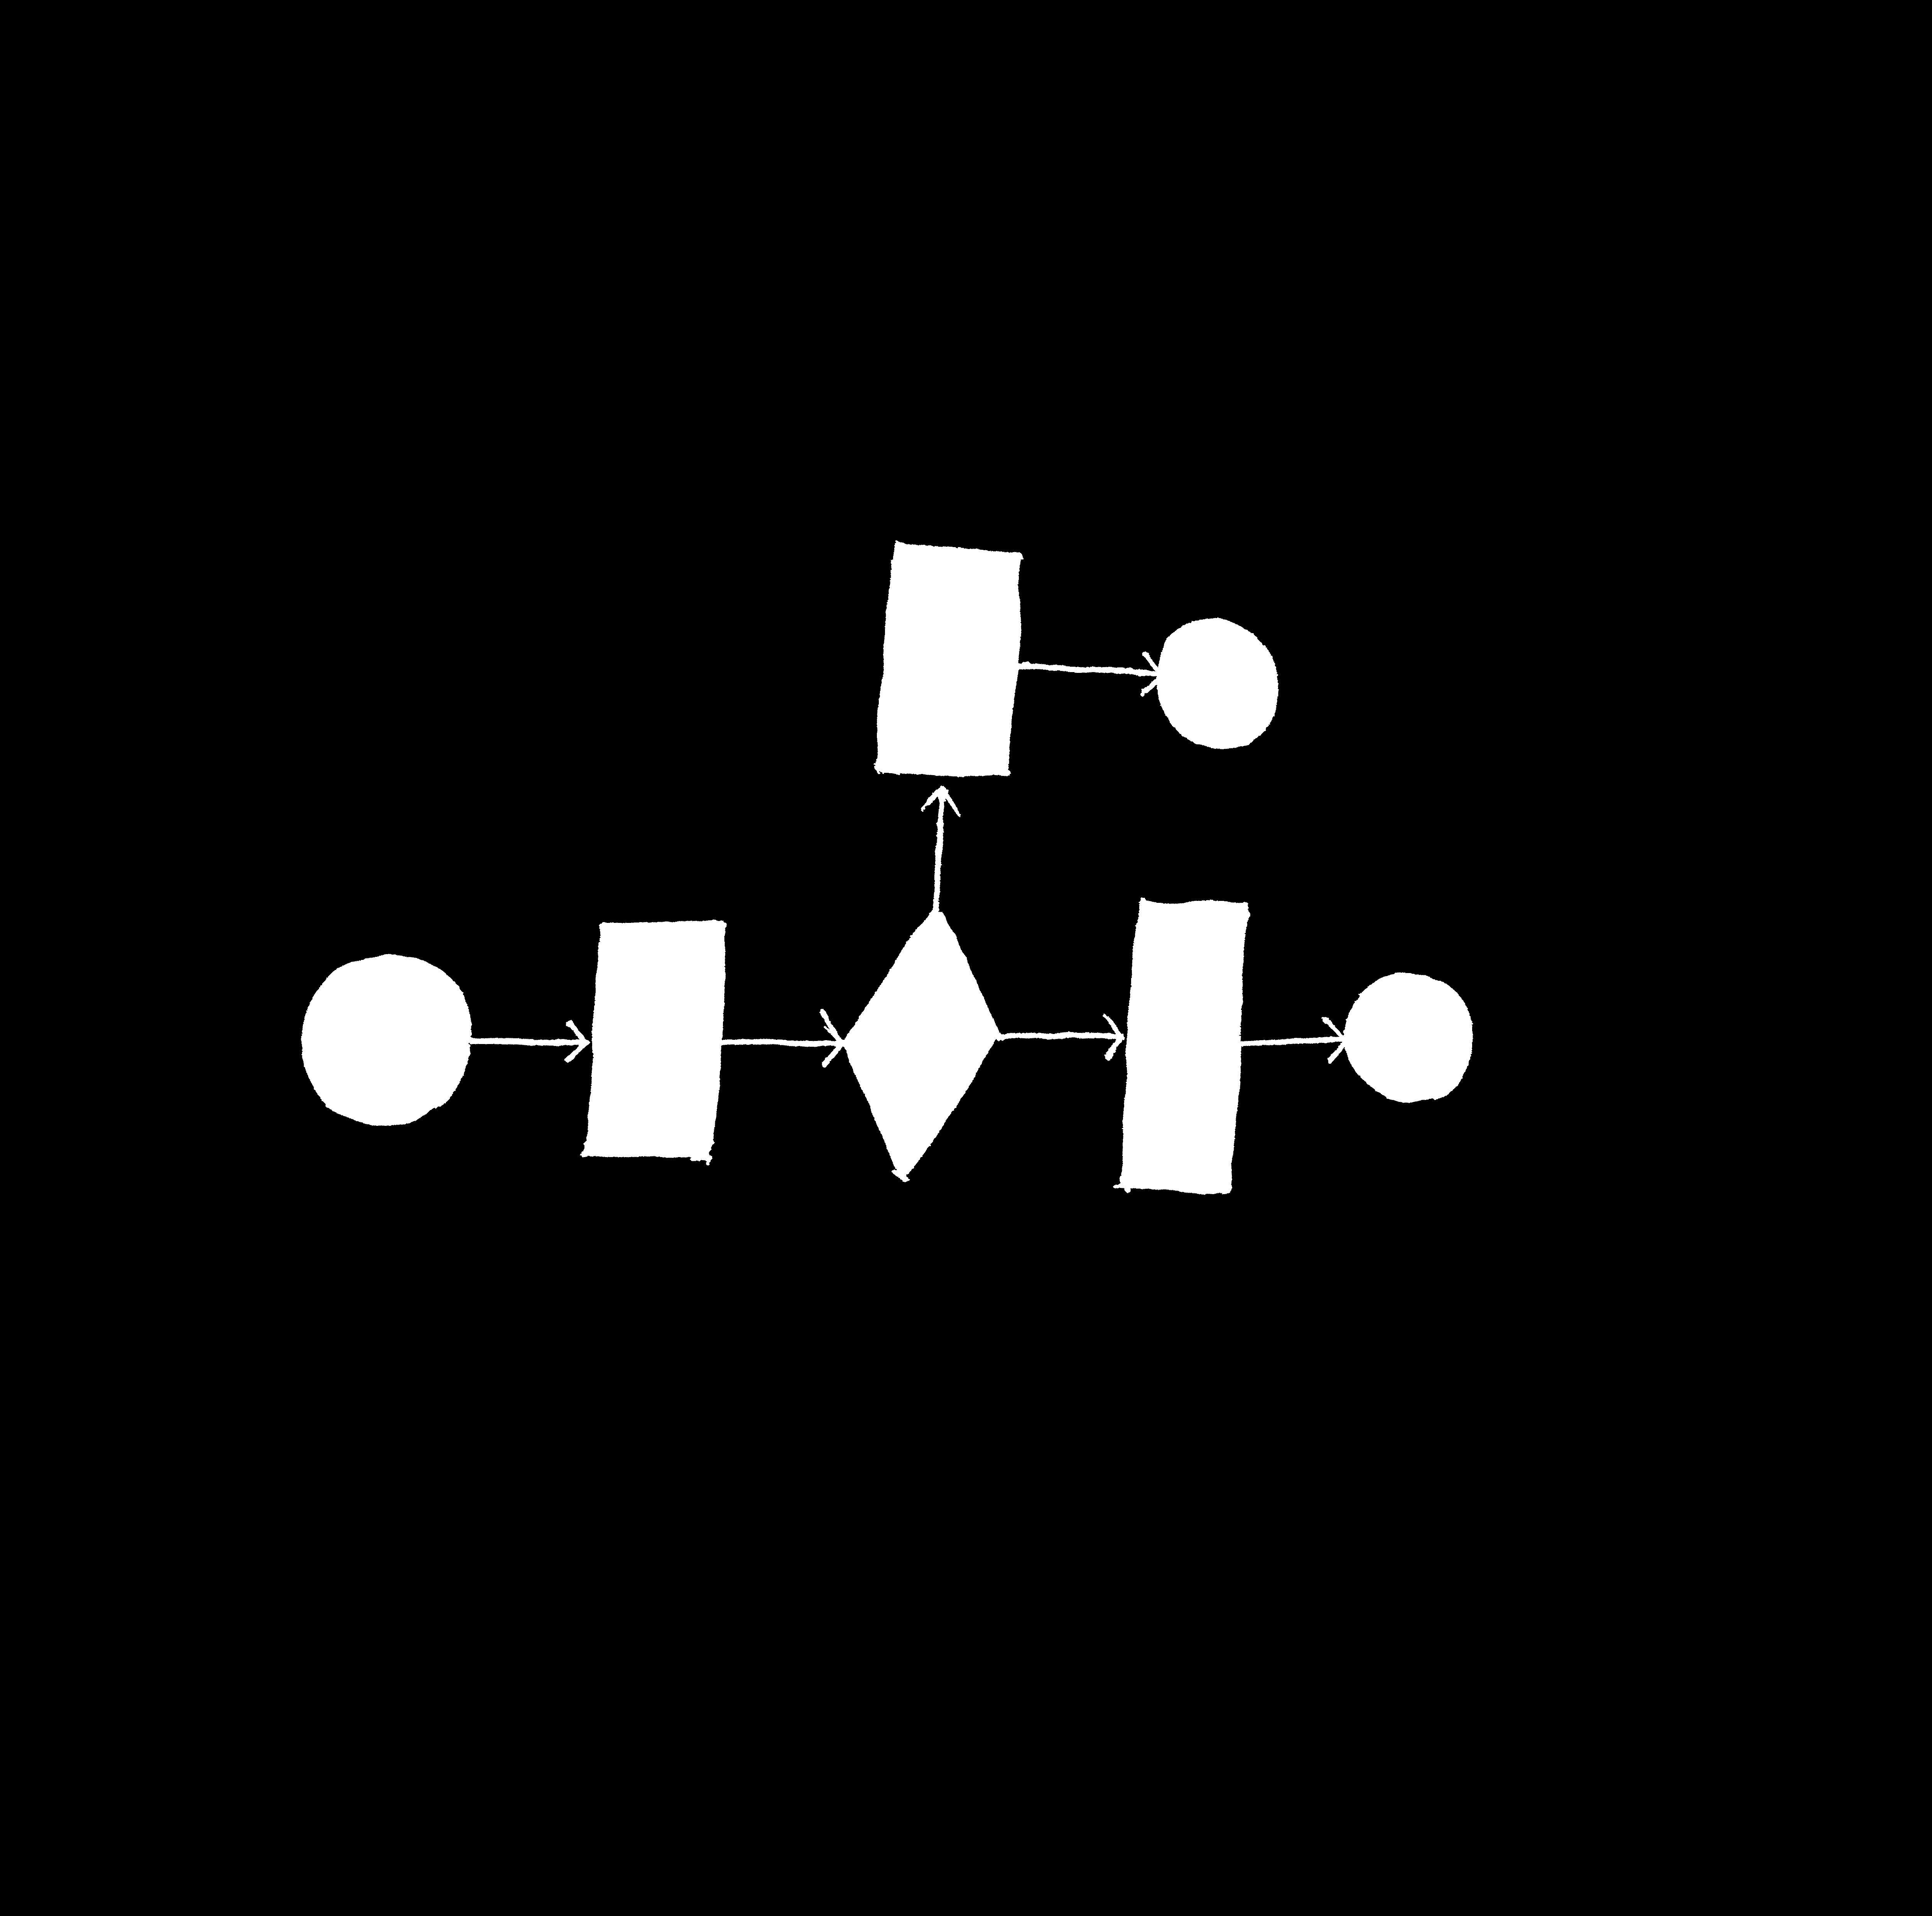
\includegraphics[height=4.8cm, angle=270]{fig/fill.png}
    }
    \caption{Shift and Rotation}
    \label{fig:rotation}
\end{figure}



\subsubsection{Decomposition}
To decompose the flow chart, the key is to separate arrows from shapes in the chart. Since we have already filled the contours with white color, what is now in the image is only arrows and filled shapes. First, we apply an "open" filter to the image, which erodes the white area and remove arrows from the image, then dilates to recover the shapes to their original size, as shown in Fig~\ref{fig:open}. Second, subtract these shapes from the original image, thus we get the arrows. Third, subtract these arrows from the original image in the same way, thus we get the shapes. However, after subtractions we find that the corners of the shapes are left in the image due to the edge effect caused by open operation. Therefore, we perform small region removal algorithm one more time, to eliminate those small white areas with an appropriate threshold. The result is shown in Fig~\ref{fig:extract}.

\begin{figure}[!htbp]
    \centering
    \subfigure[Before Opening Operation]
    {
        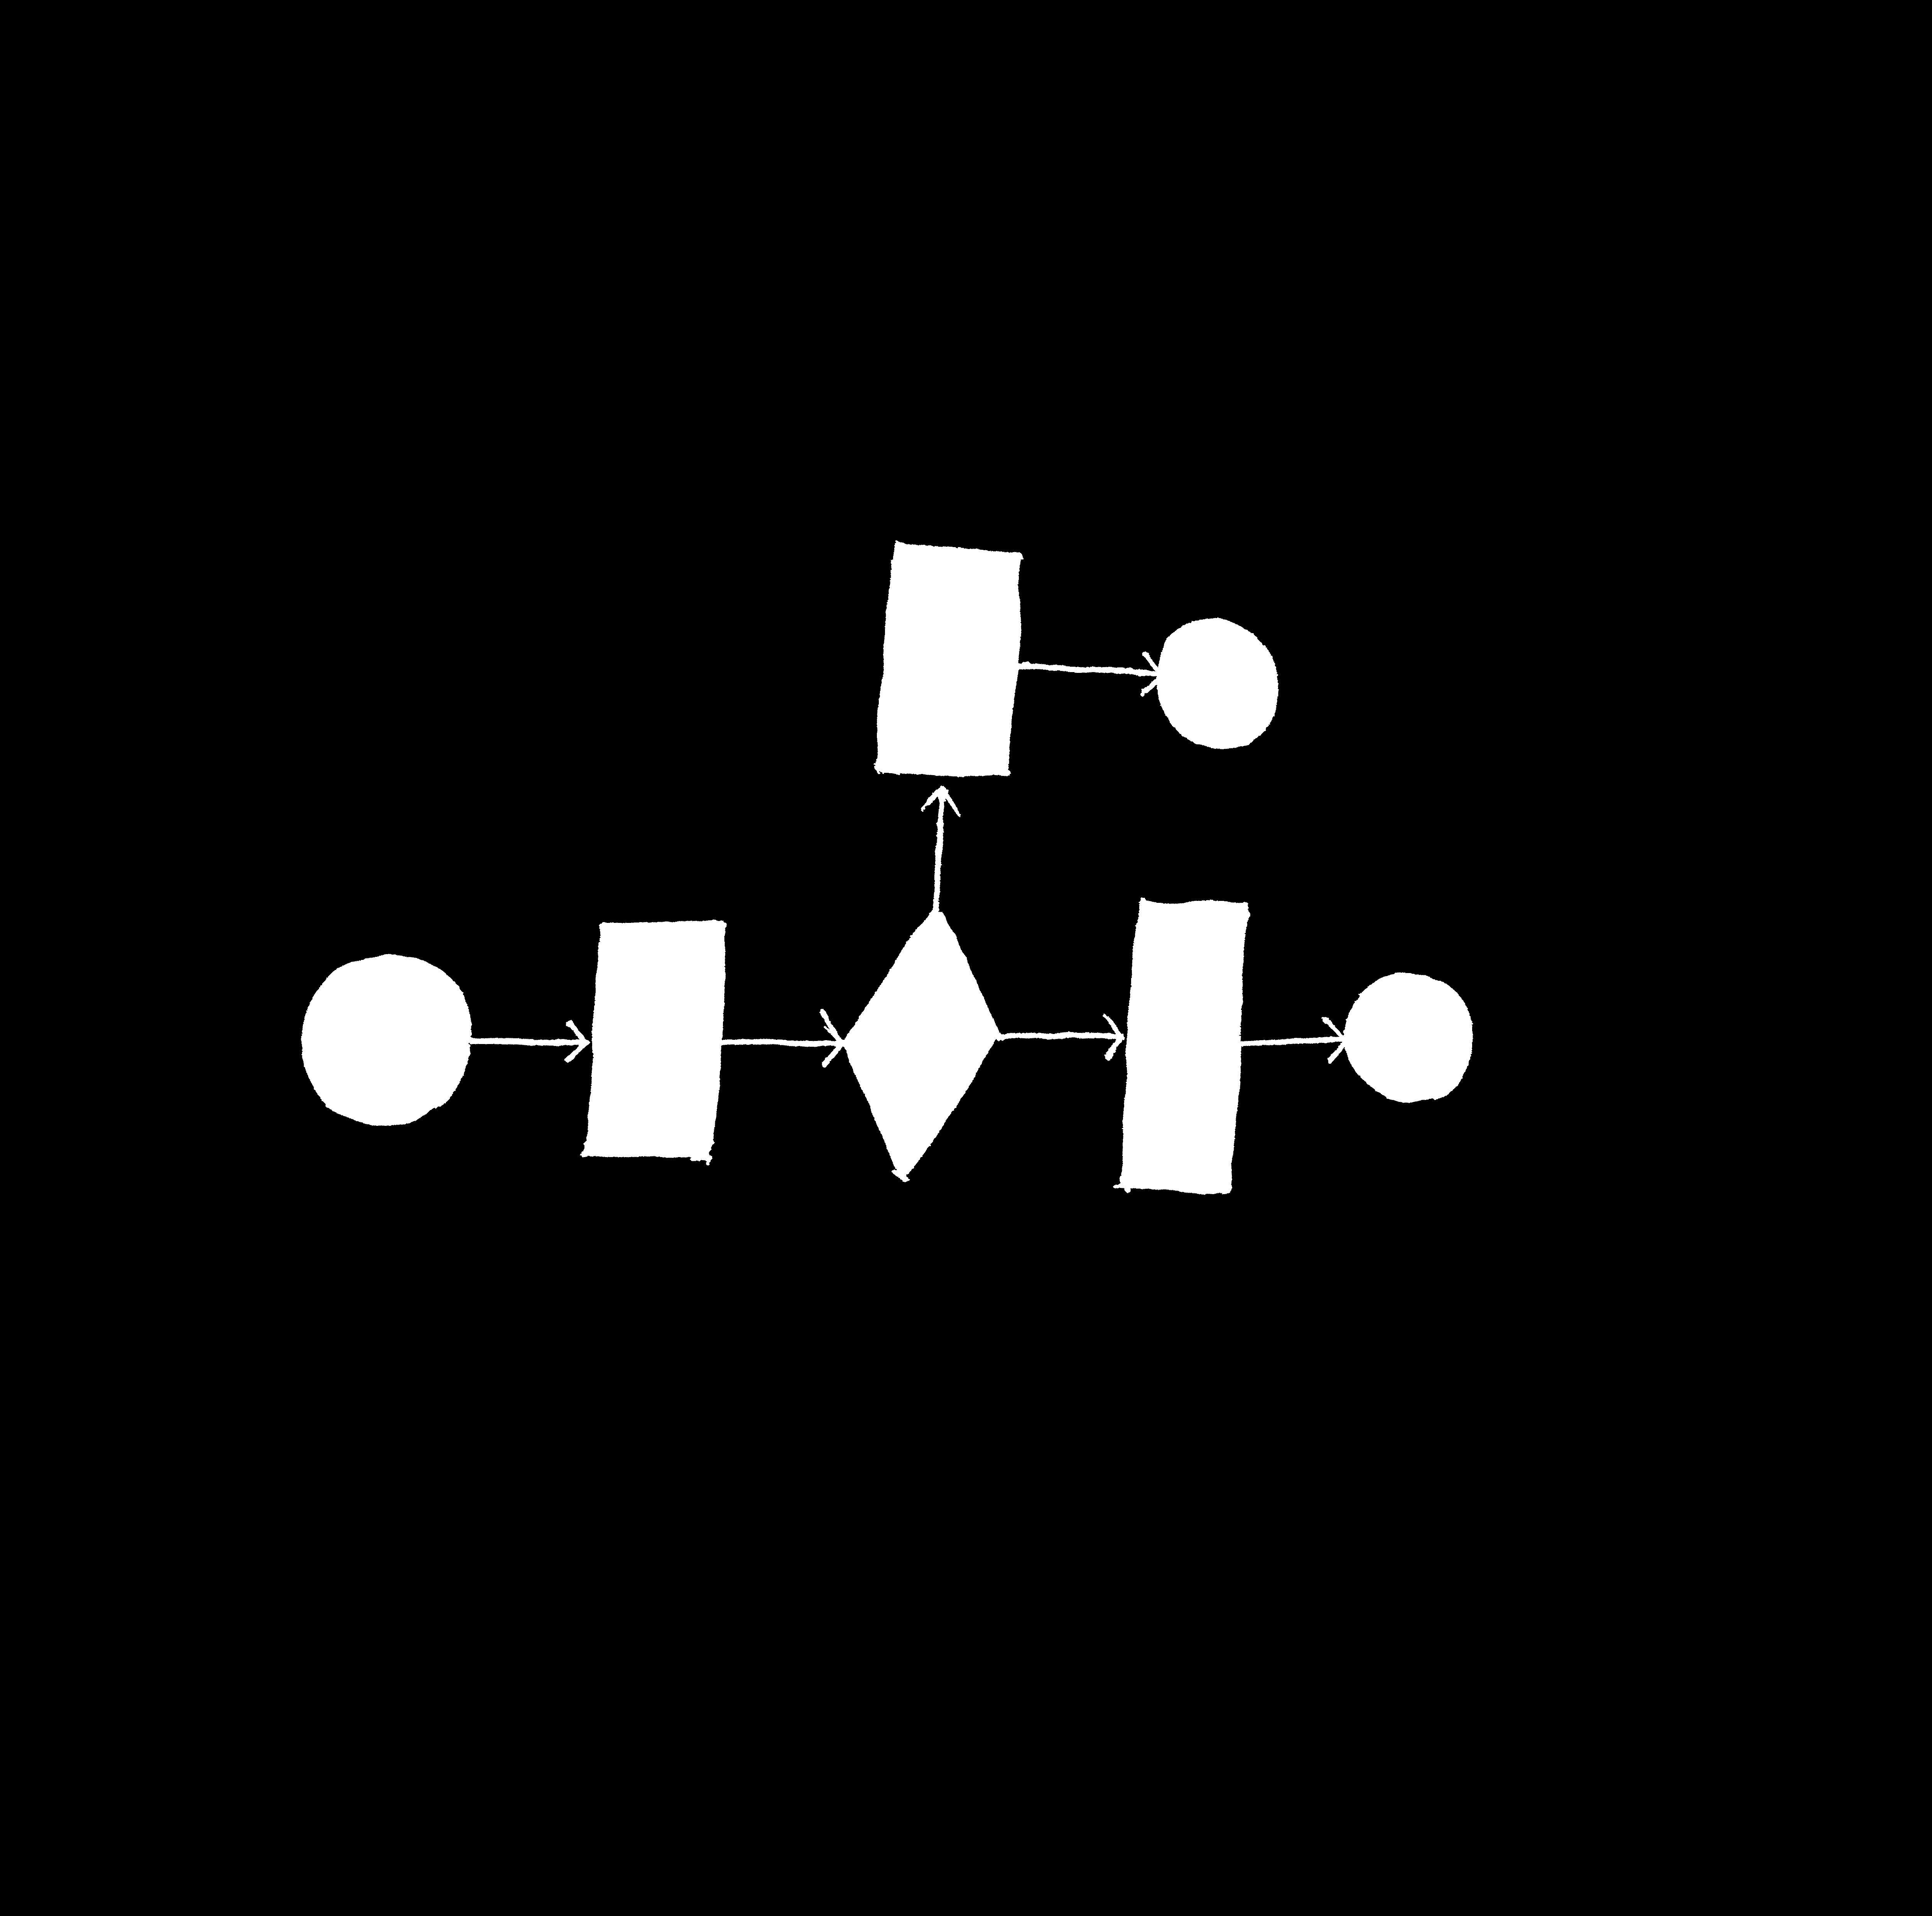
\includegraphics[angle=270, width=0.2\textwidth]{fig/fill.png}
    }
    \subfigure[After Opening Operation]
    {
        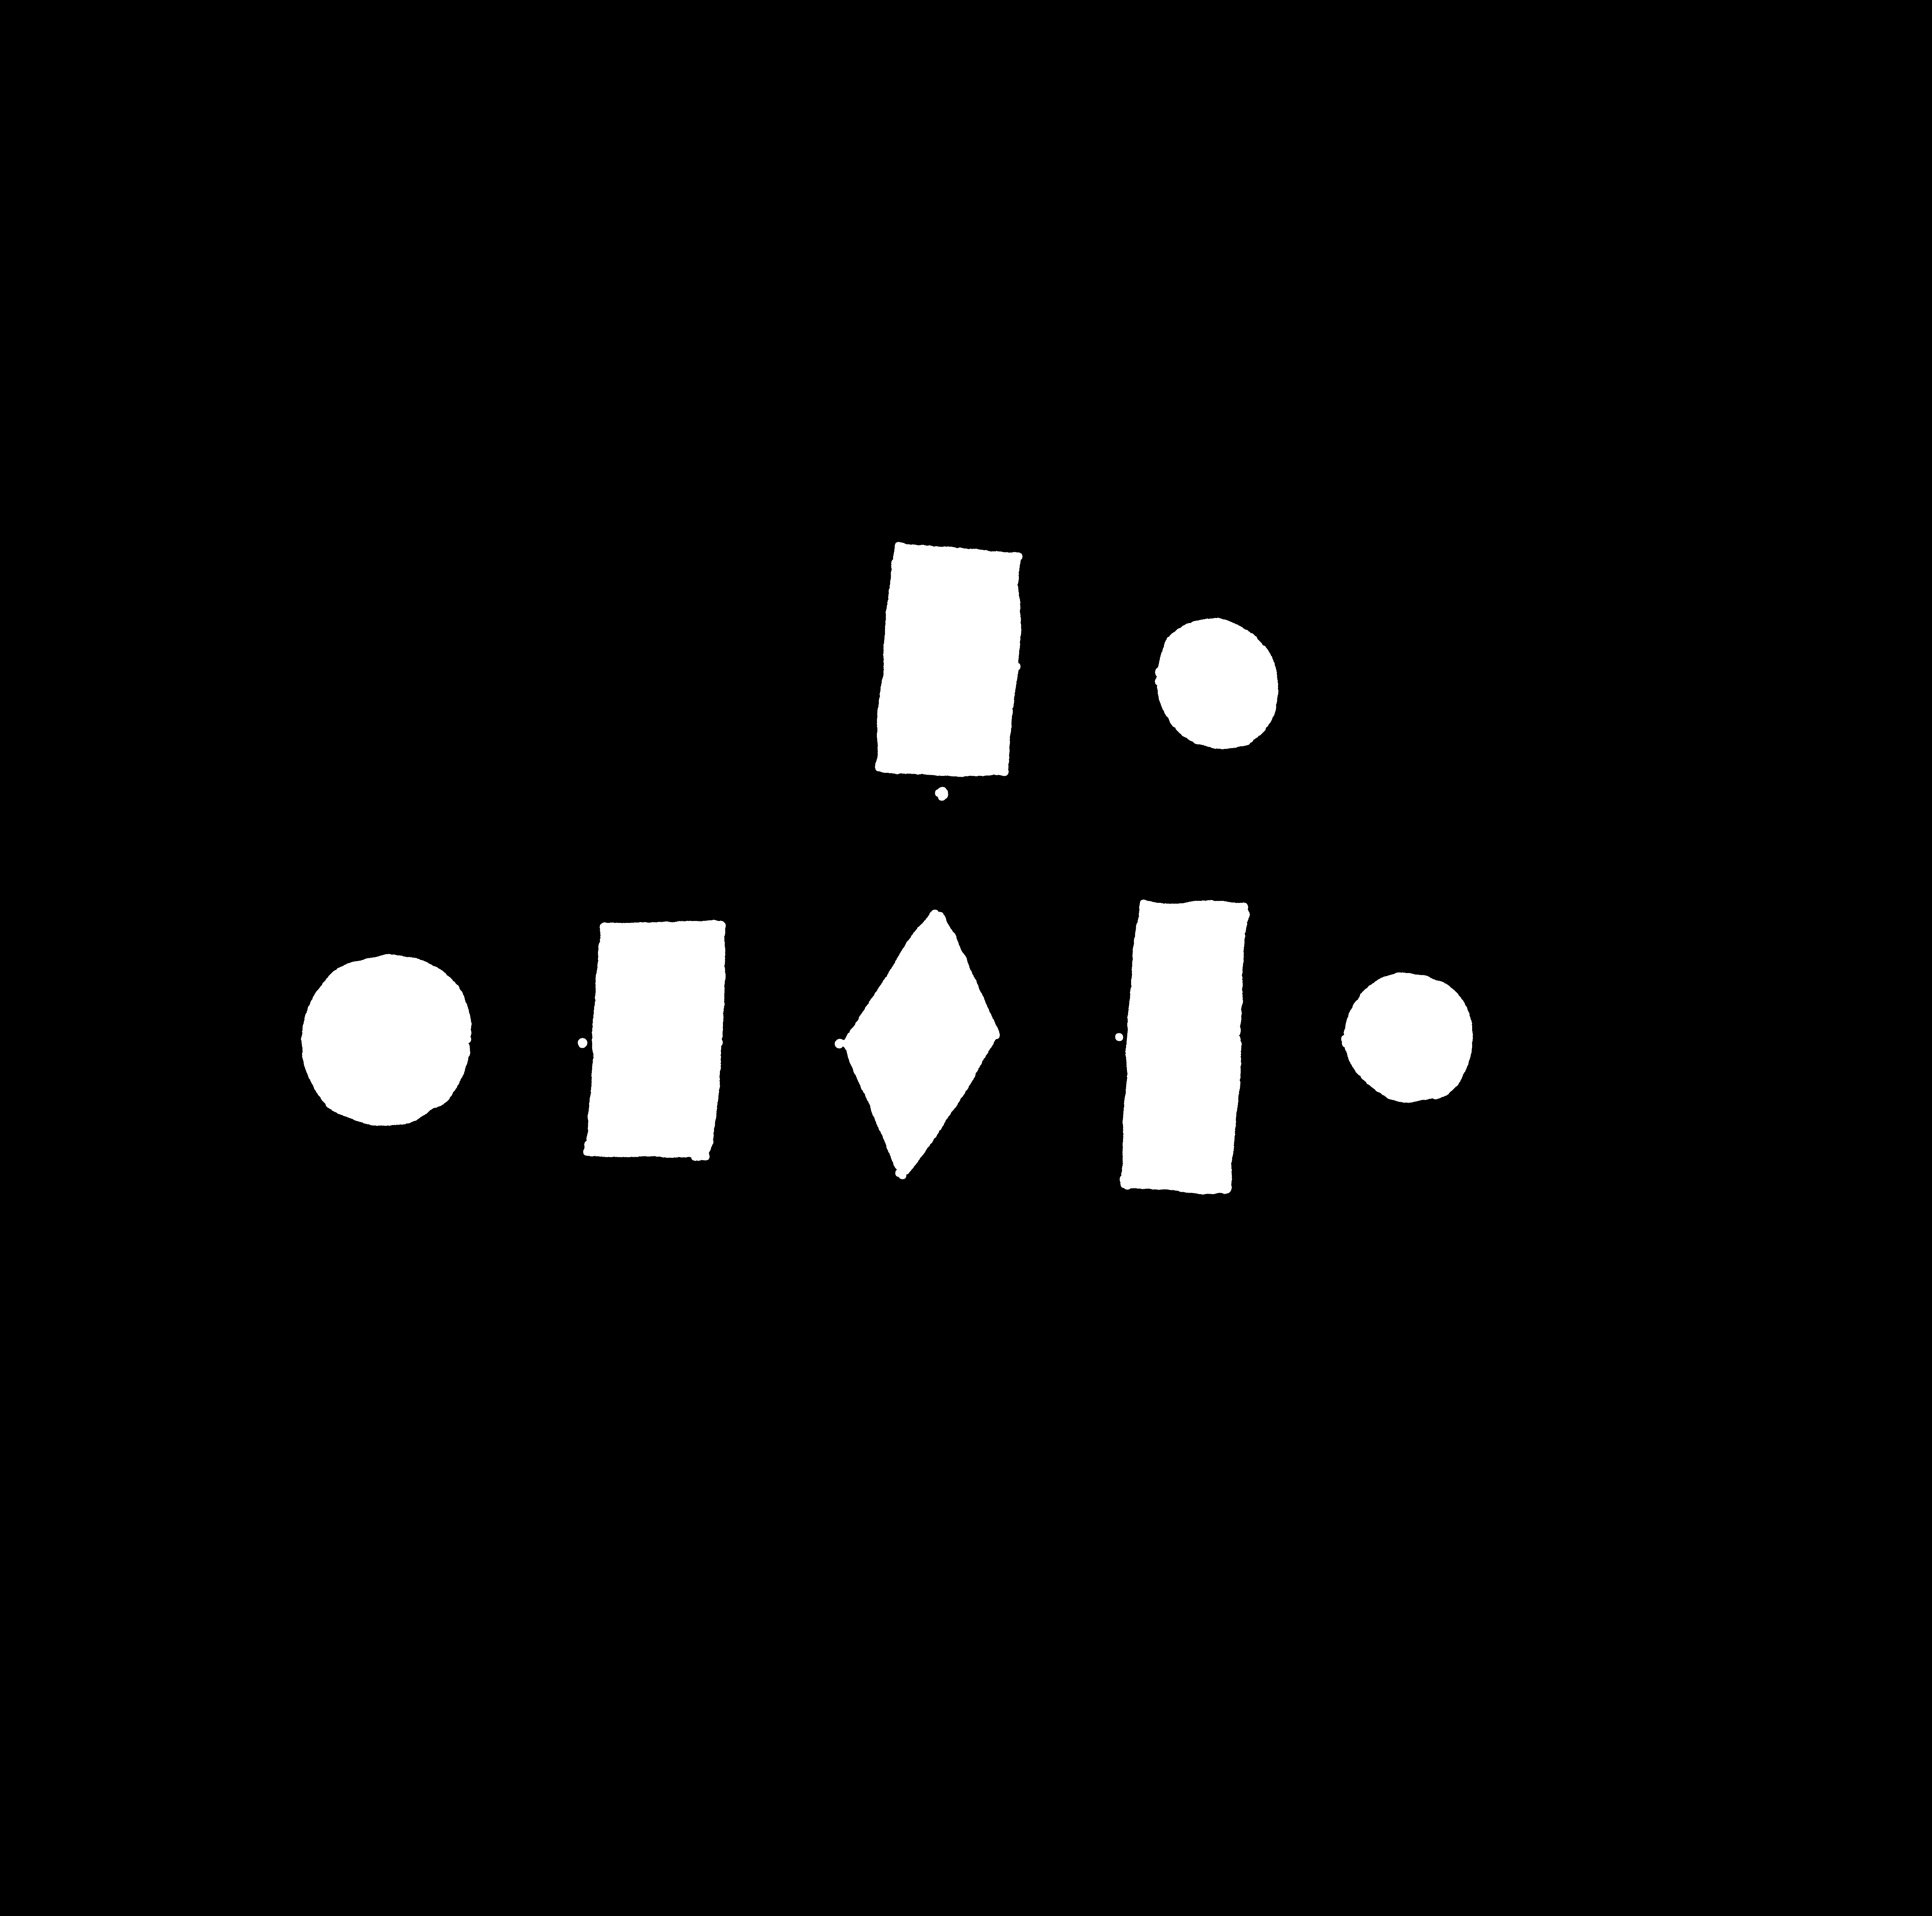
\includegraphics[angle=270, width=0.2\textwidth]{fig/open.png}
    }
    \caption{Opening Operation}
    \label{fig:open}
\end{figure}

\begin{figure}[!htbp]
    \centering
    \subfigure[Extracted Arrows]
    {
        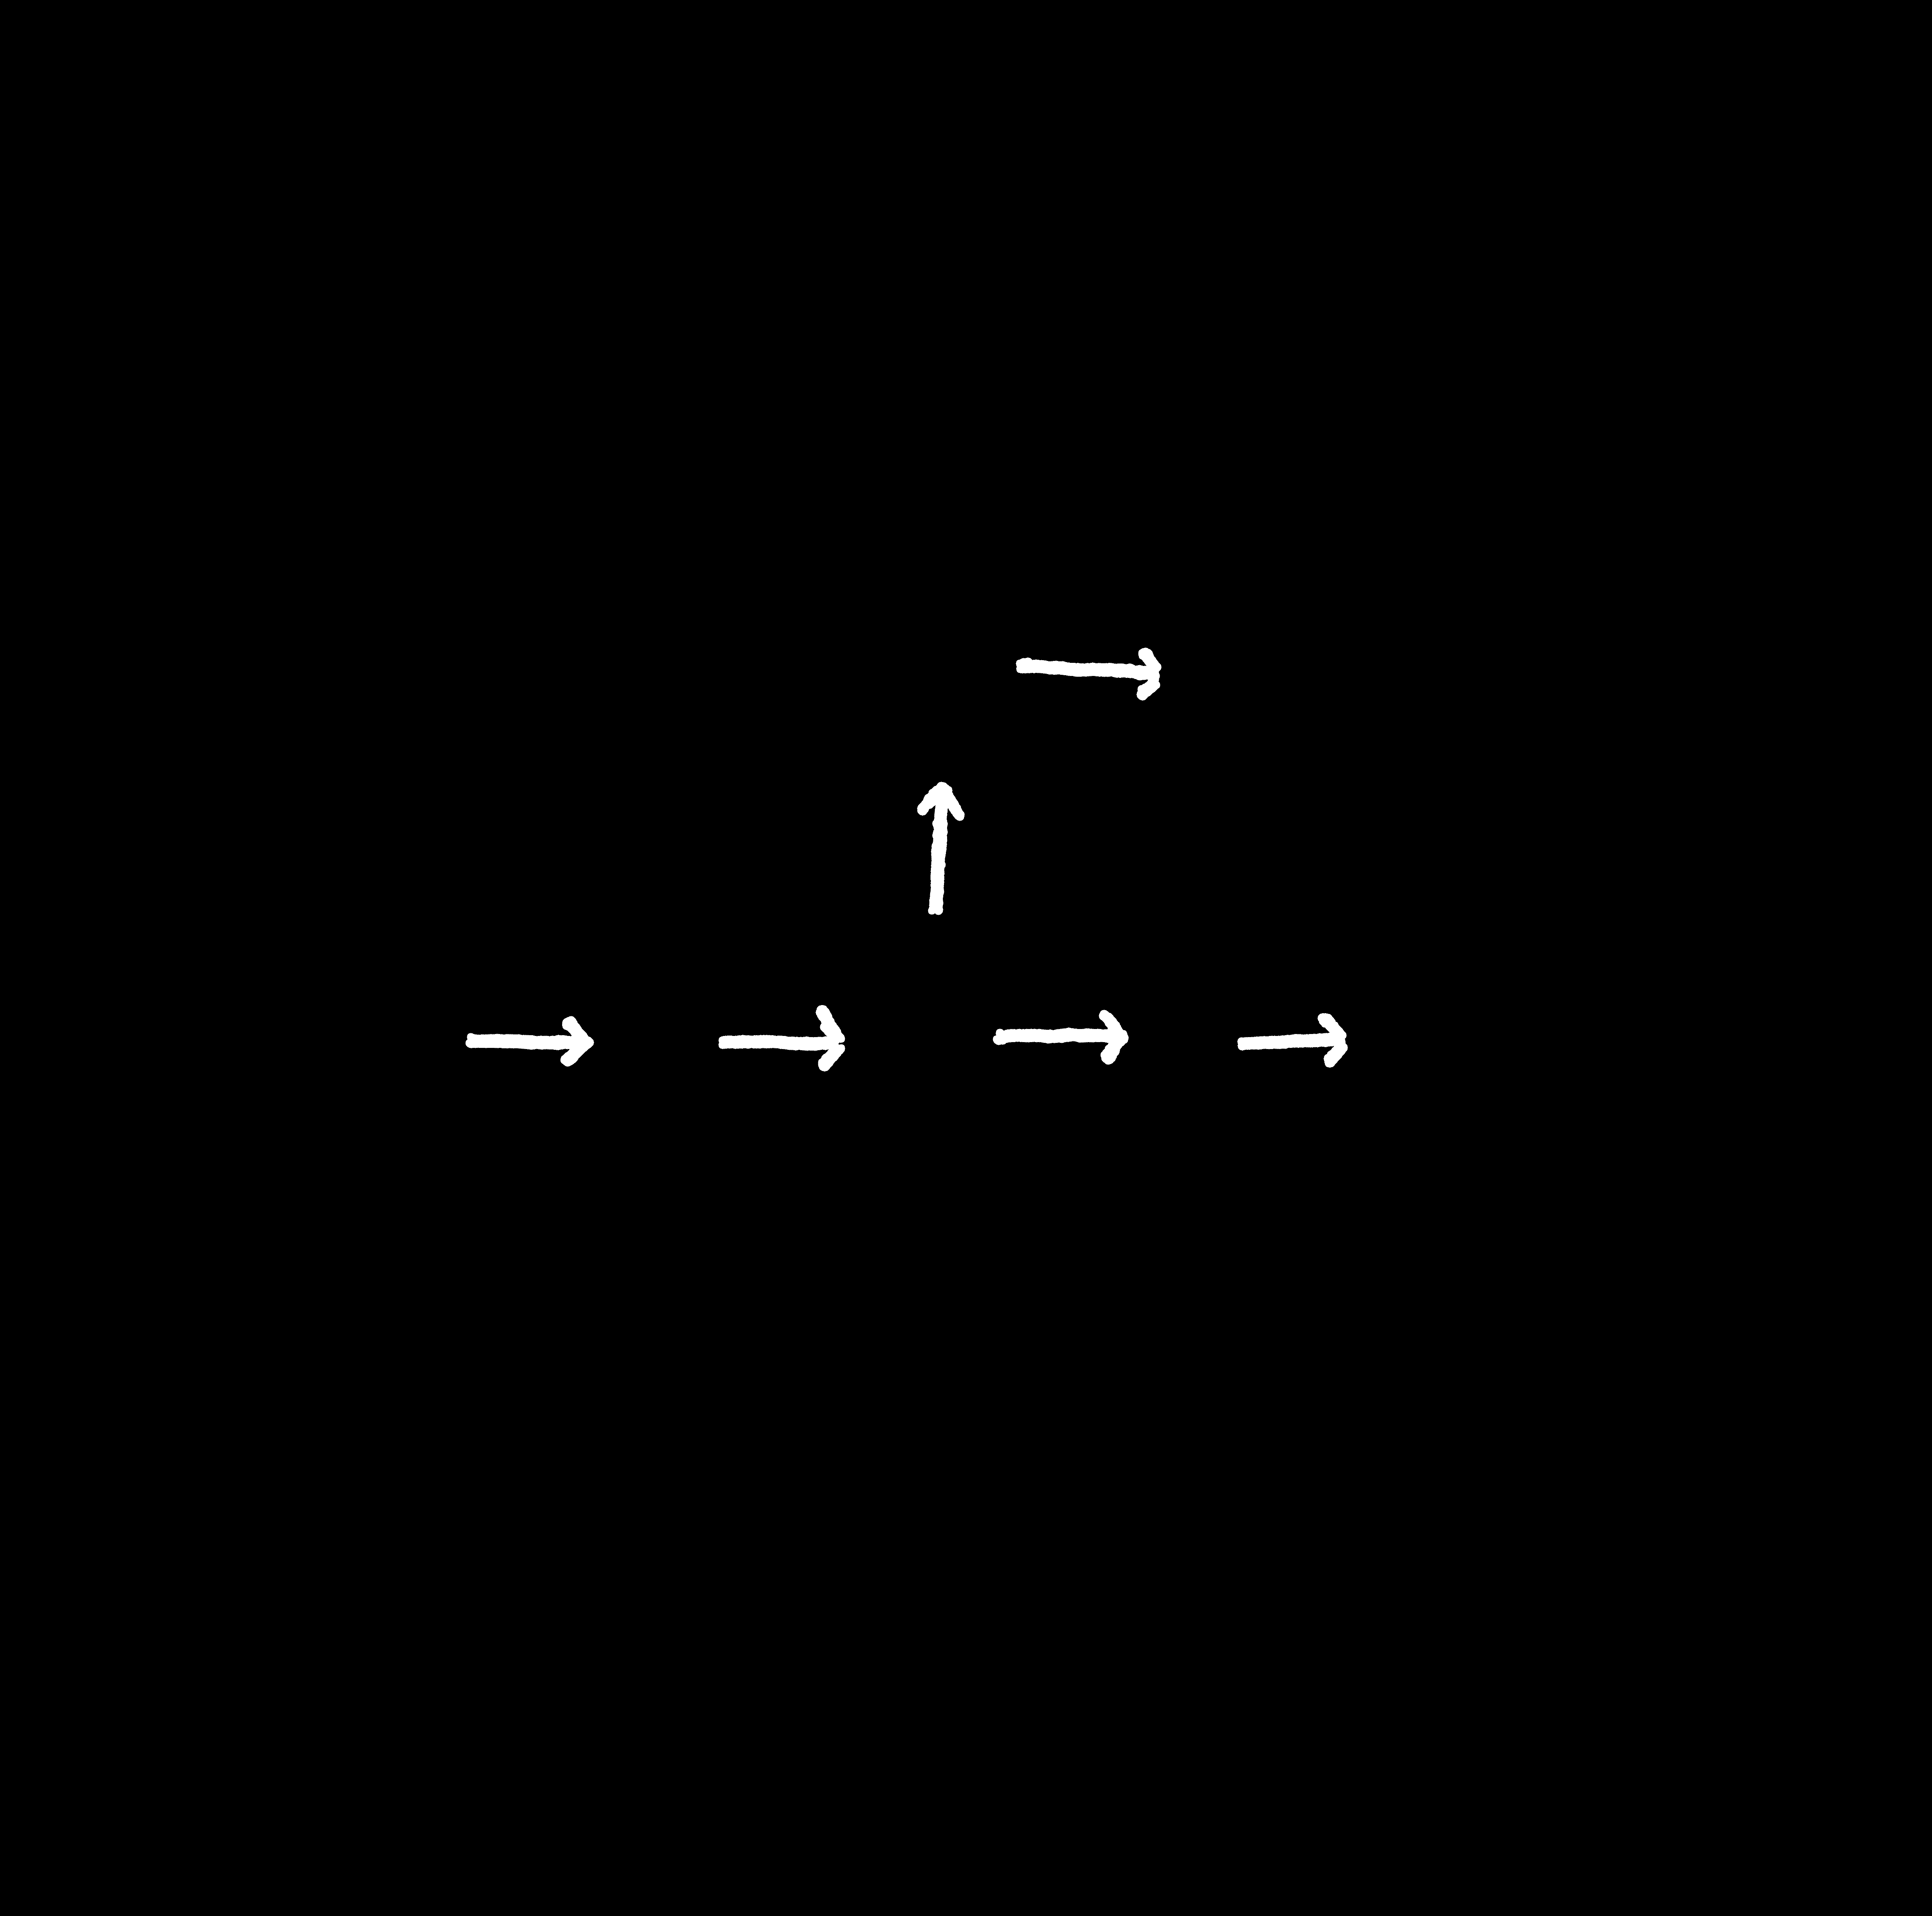
\includegraphics[angle=270, width=0.2\textwidth]{fig/arrows.png}
    }
    \subfigure[Extracted Shapes]
    {
        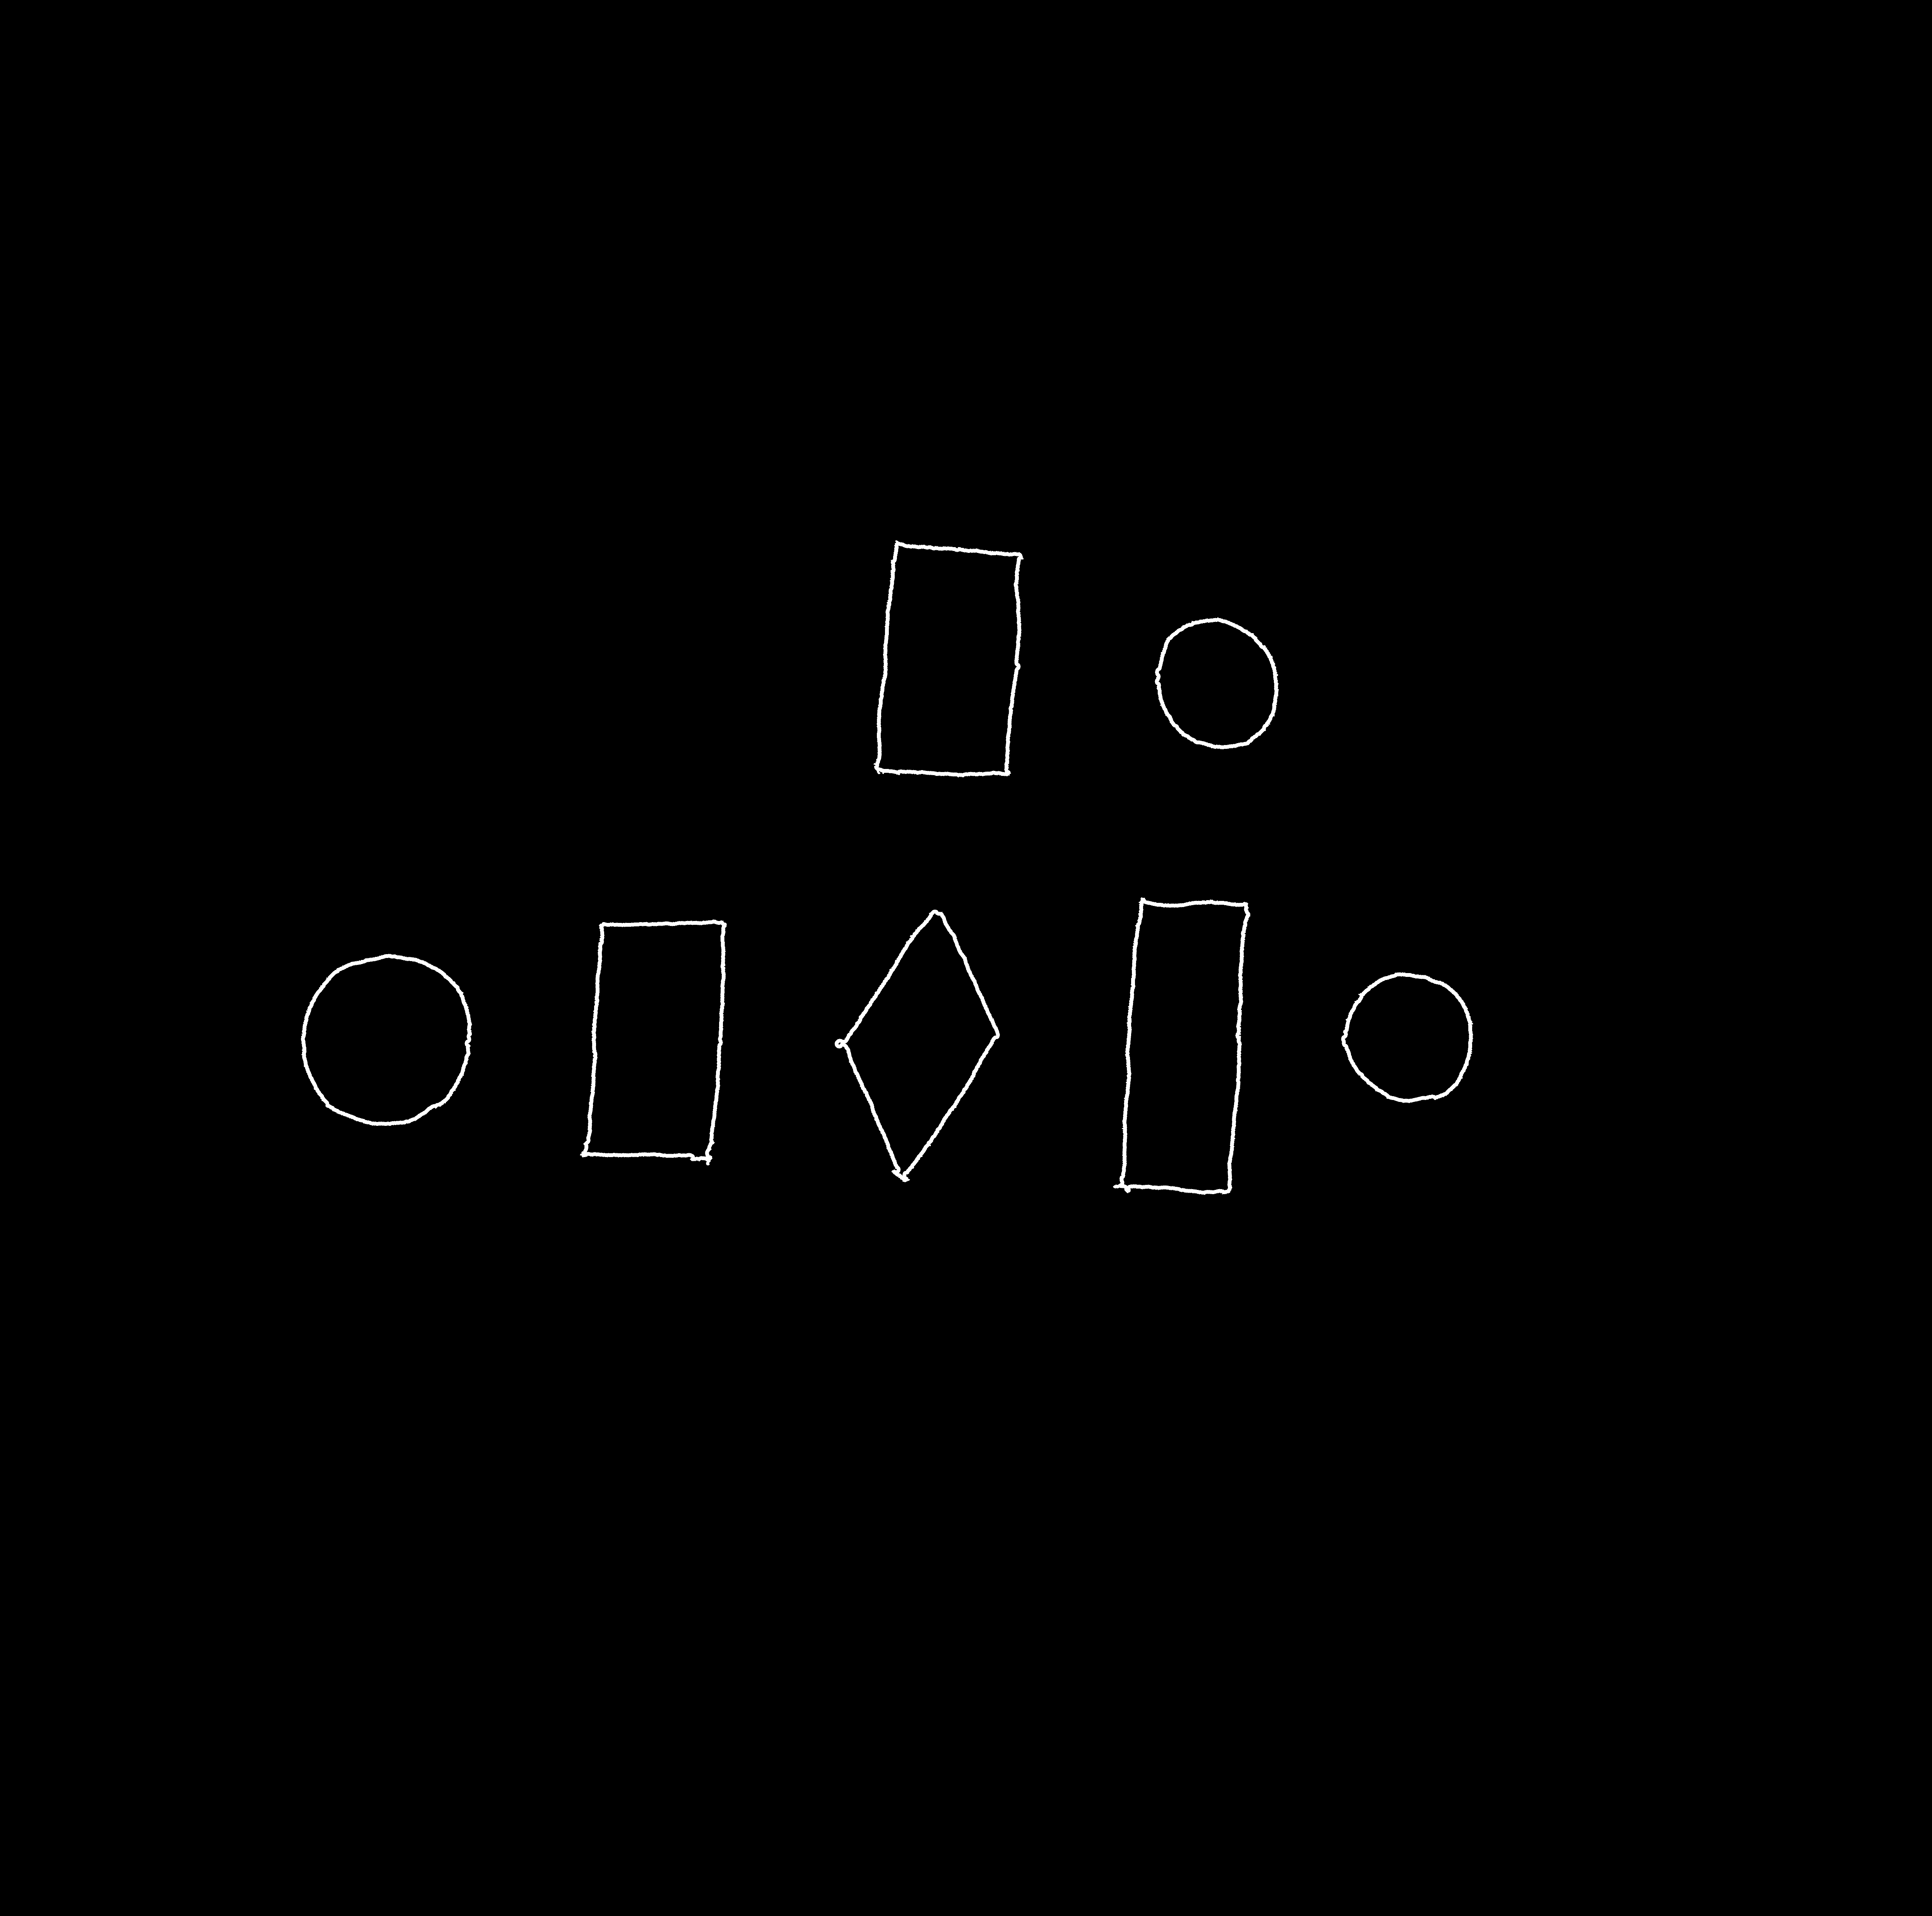
\includegraphics[angle=270, width=0.2\textwidth]{fig/diff_blob.png}
    }
    \caption{Extracted Arrows and Shapes}
    \label{fig:extract}
\end{figure}


\subsubsection{Classification}
    
    After all the components are disconnected after decomposition step, we found and labeled the connected ones to determine the regions of each shape. With \emph{OpenCV.connectedComponentsWithStats}, we are able to label and get the centroids of the components, as well as the boundary box of each component. First, circles are differentiated from the other shapes by \emph{OpenCV.HoughCircles}, as shown in Fig~\ref{fig:circ}. Next, diamonds can be identified by comparing the ratio between the area of each shape and the area of the boundary box. If the ratio is close to 1, this means the shape is a rectangle. On the other hand, if the ratio is lower than 0.75, the shape would be defined as a diamond. The distinguished rectangles and circles are shown in Fig~\ref{fig:rectNdiam}.
    
\begin{figure}[!htbp]
    \centering
    \subfigure[Detected Circles]
    {
        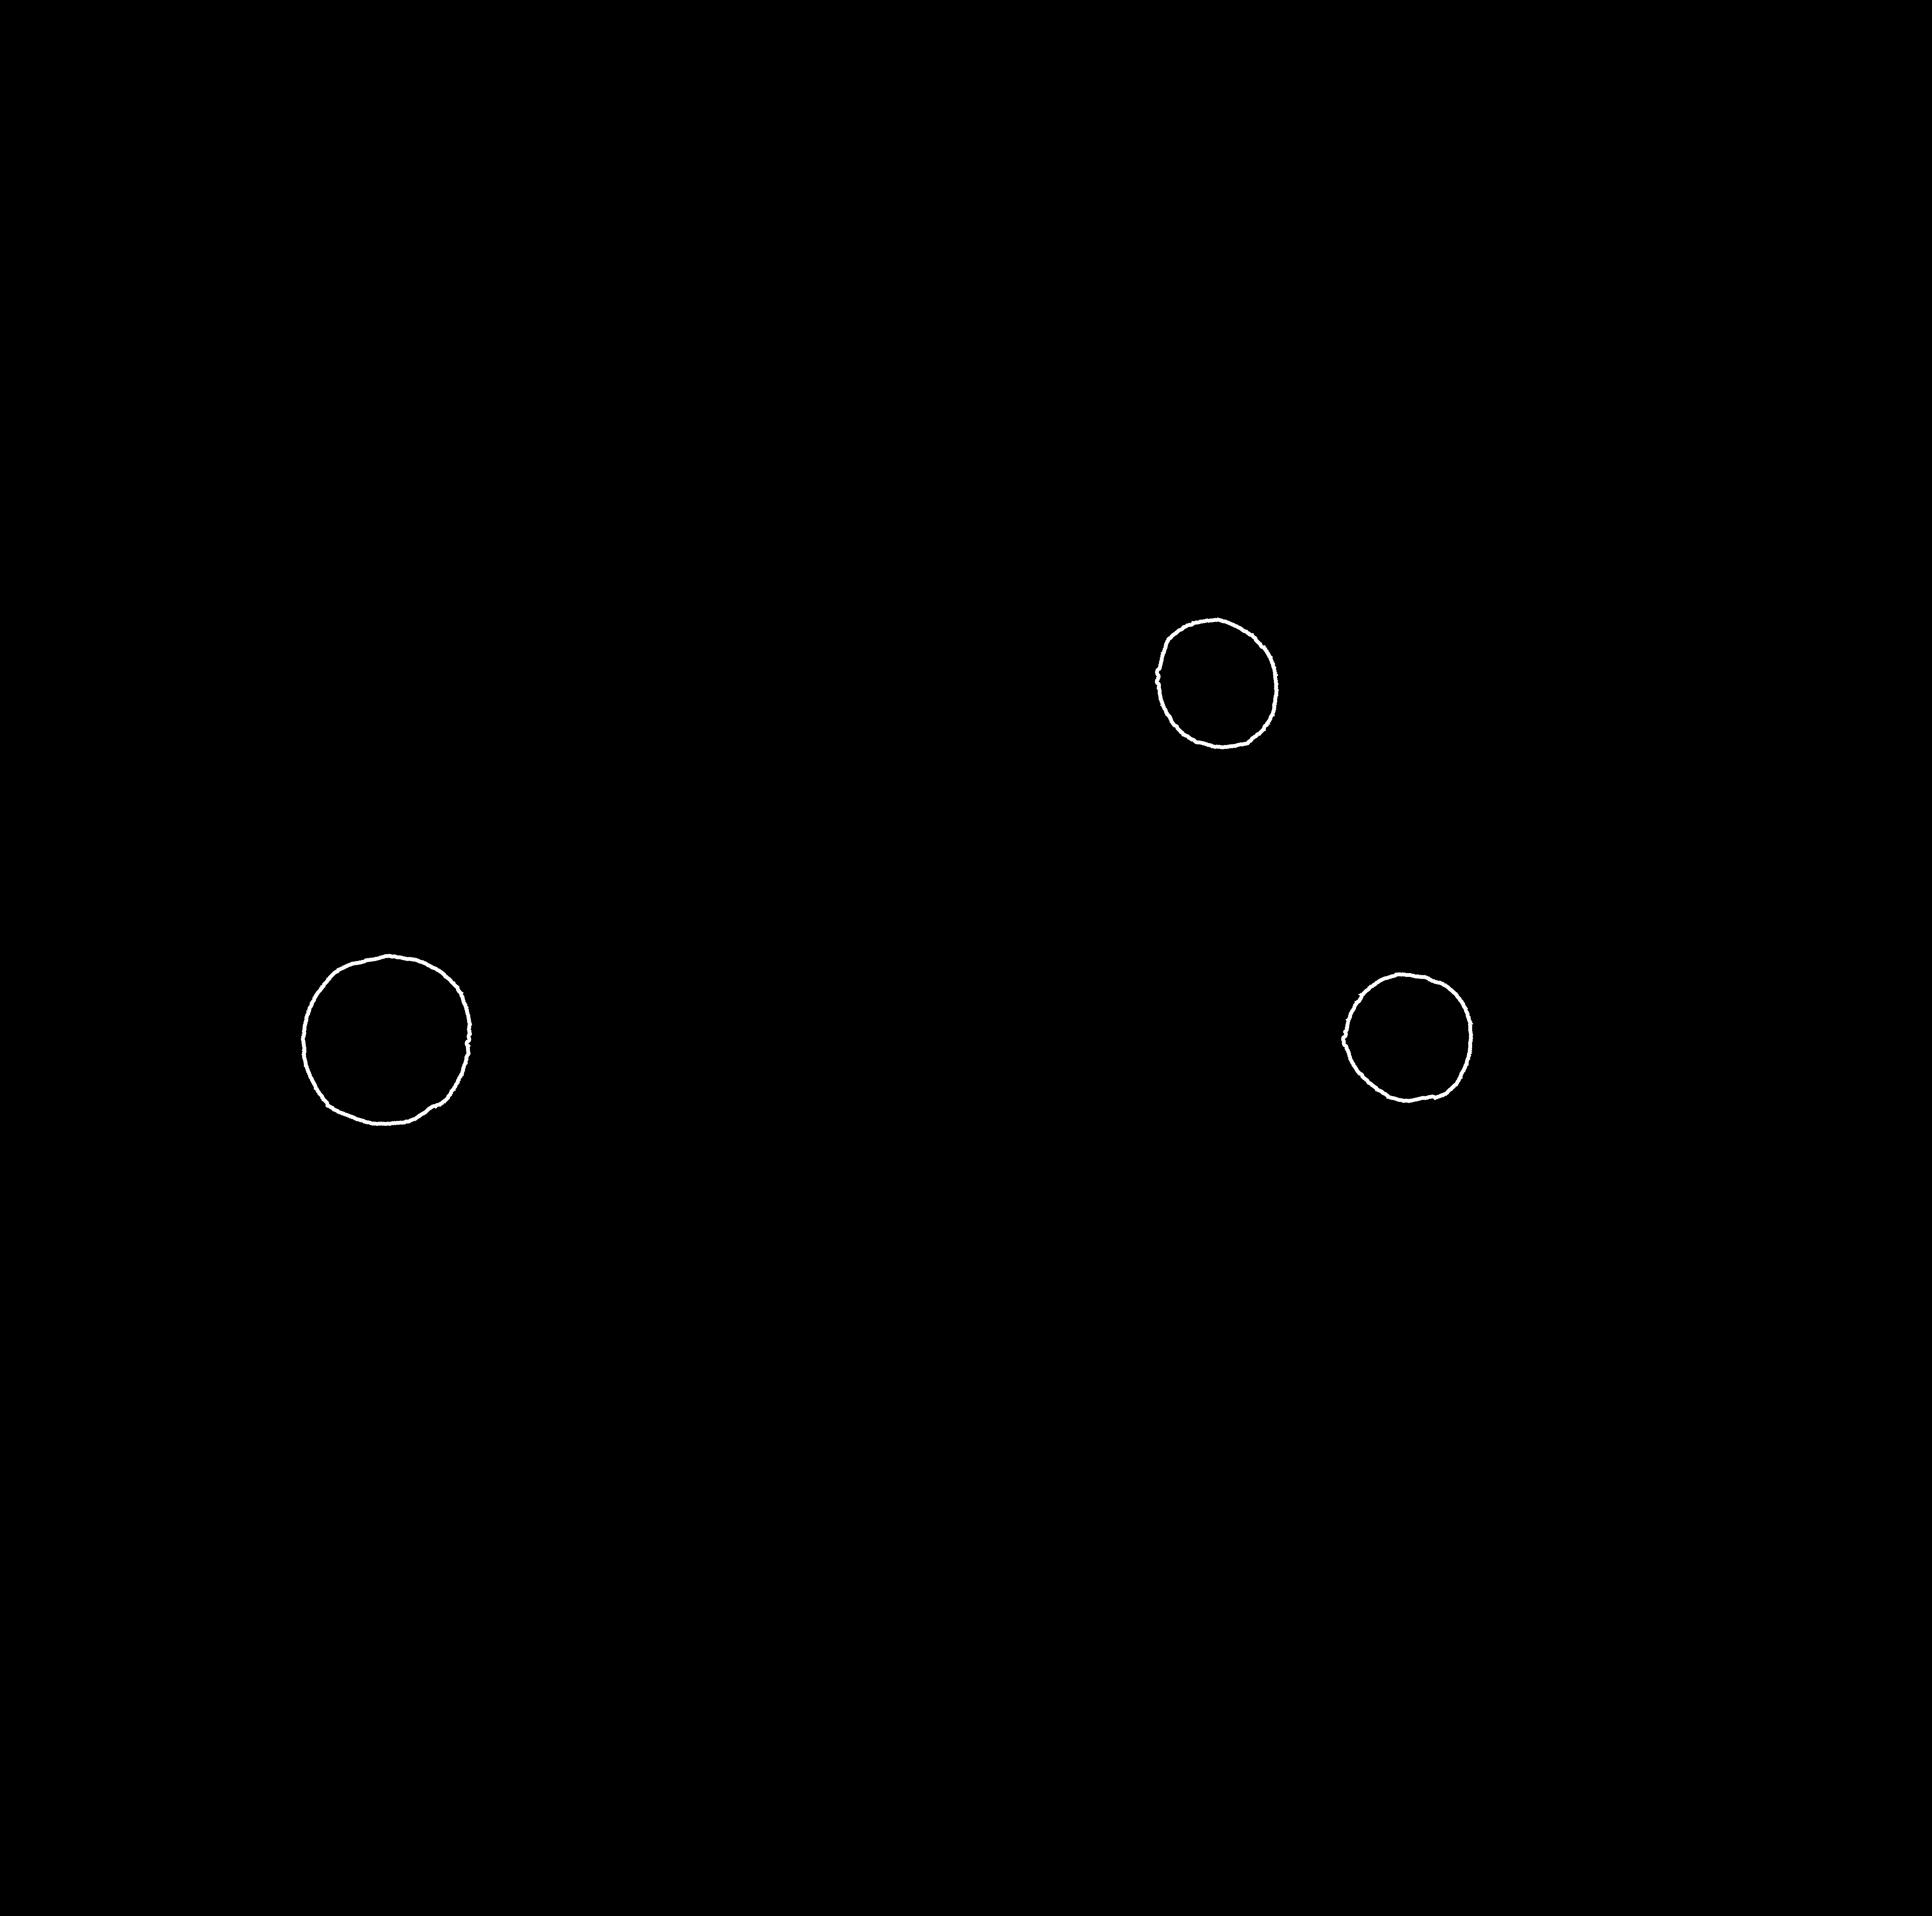
\includegraphics[angle=270, width=0.2\textwidth]{fig/circ.png}
        \label{fig:first_sub}
    }
    \subfigure[Circle Removal after Detection]
    {
        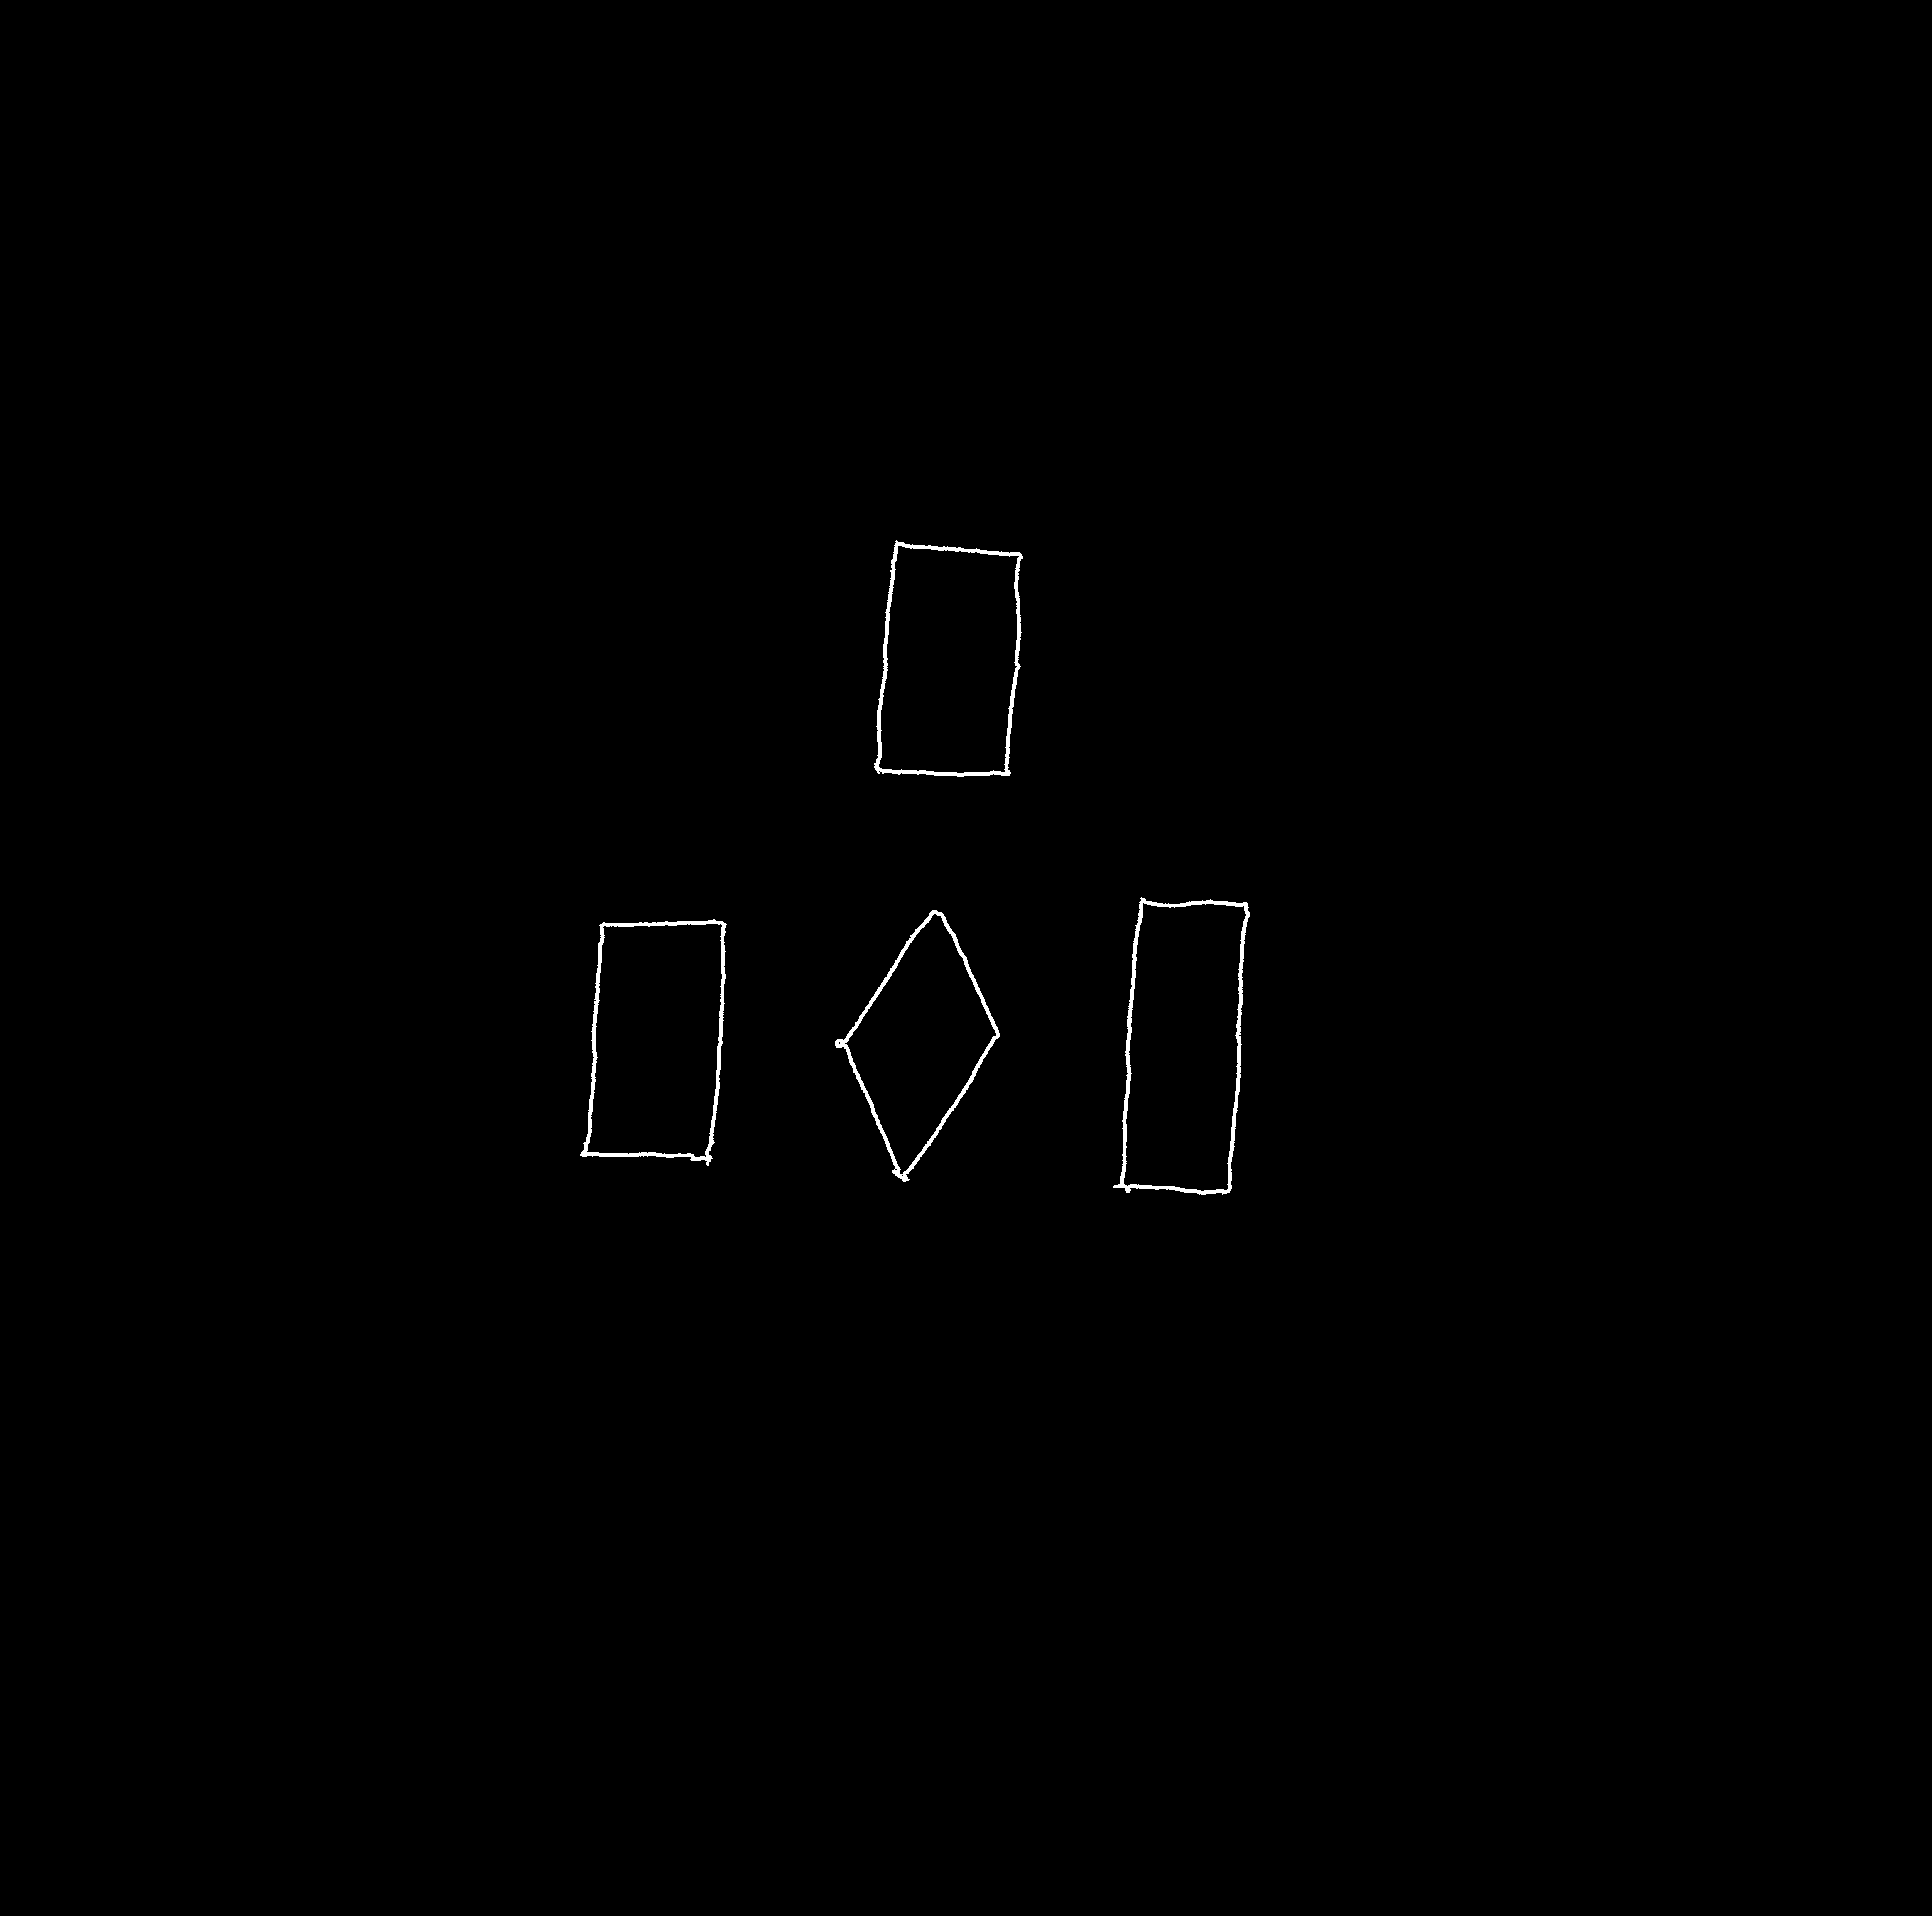
\includegraphics[angle=270, width=0.2\textwidth]{fig/copy_blob.png}
        \label{fig:second_sub}
    }
    \caption{Detected Circles and Circle Removal}
    \label{fig:circ}
\end{figure}

\begin{figure}[!htbp]
    \centering
    \subfigure[Detected Rectangles]
    {
        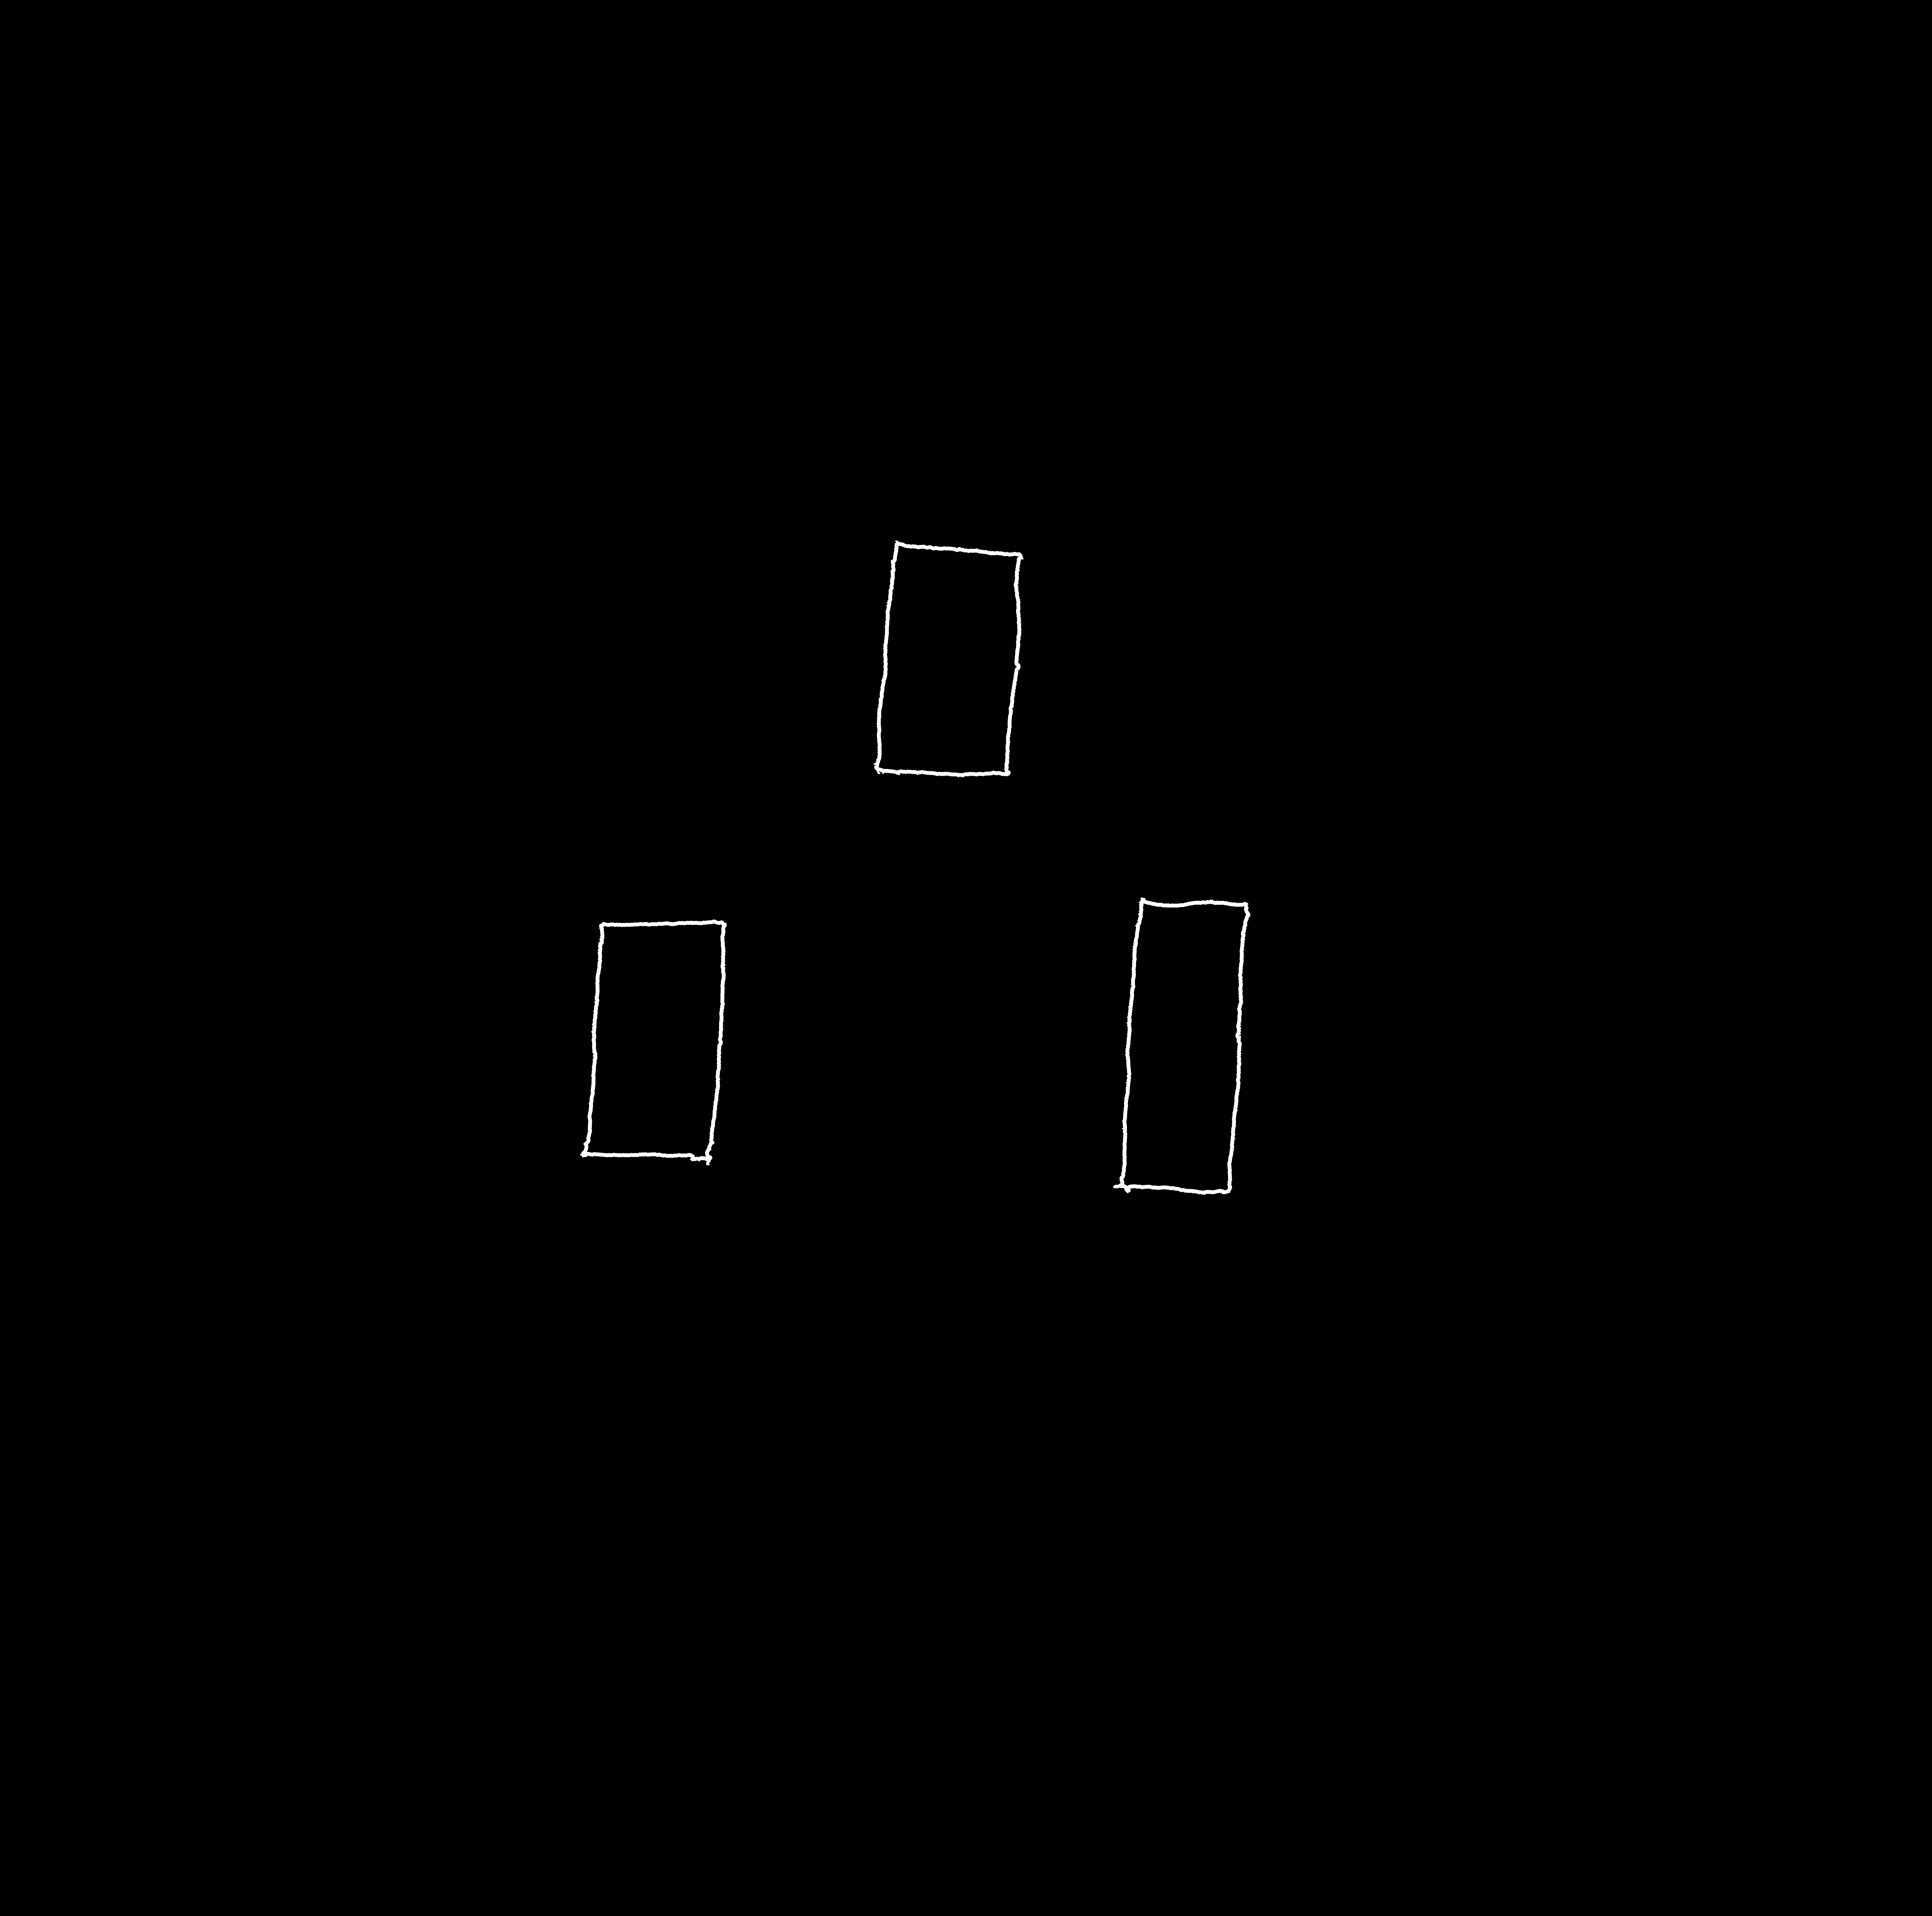
\includegraphics[angle=270, width=0.2\textwidth]{fig/rect.png}
        \label{fig:first_sub}
    }
    \subfigure[Detected Diamonds]
    {
        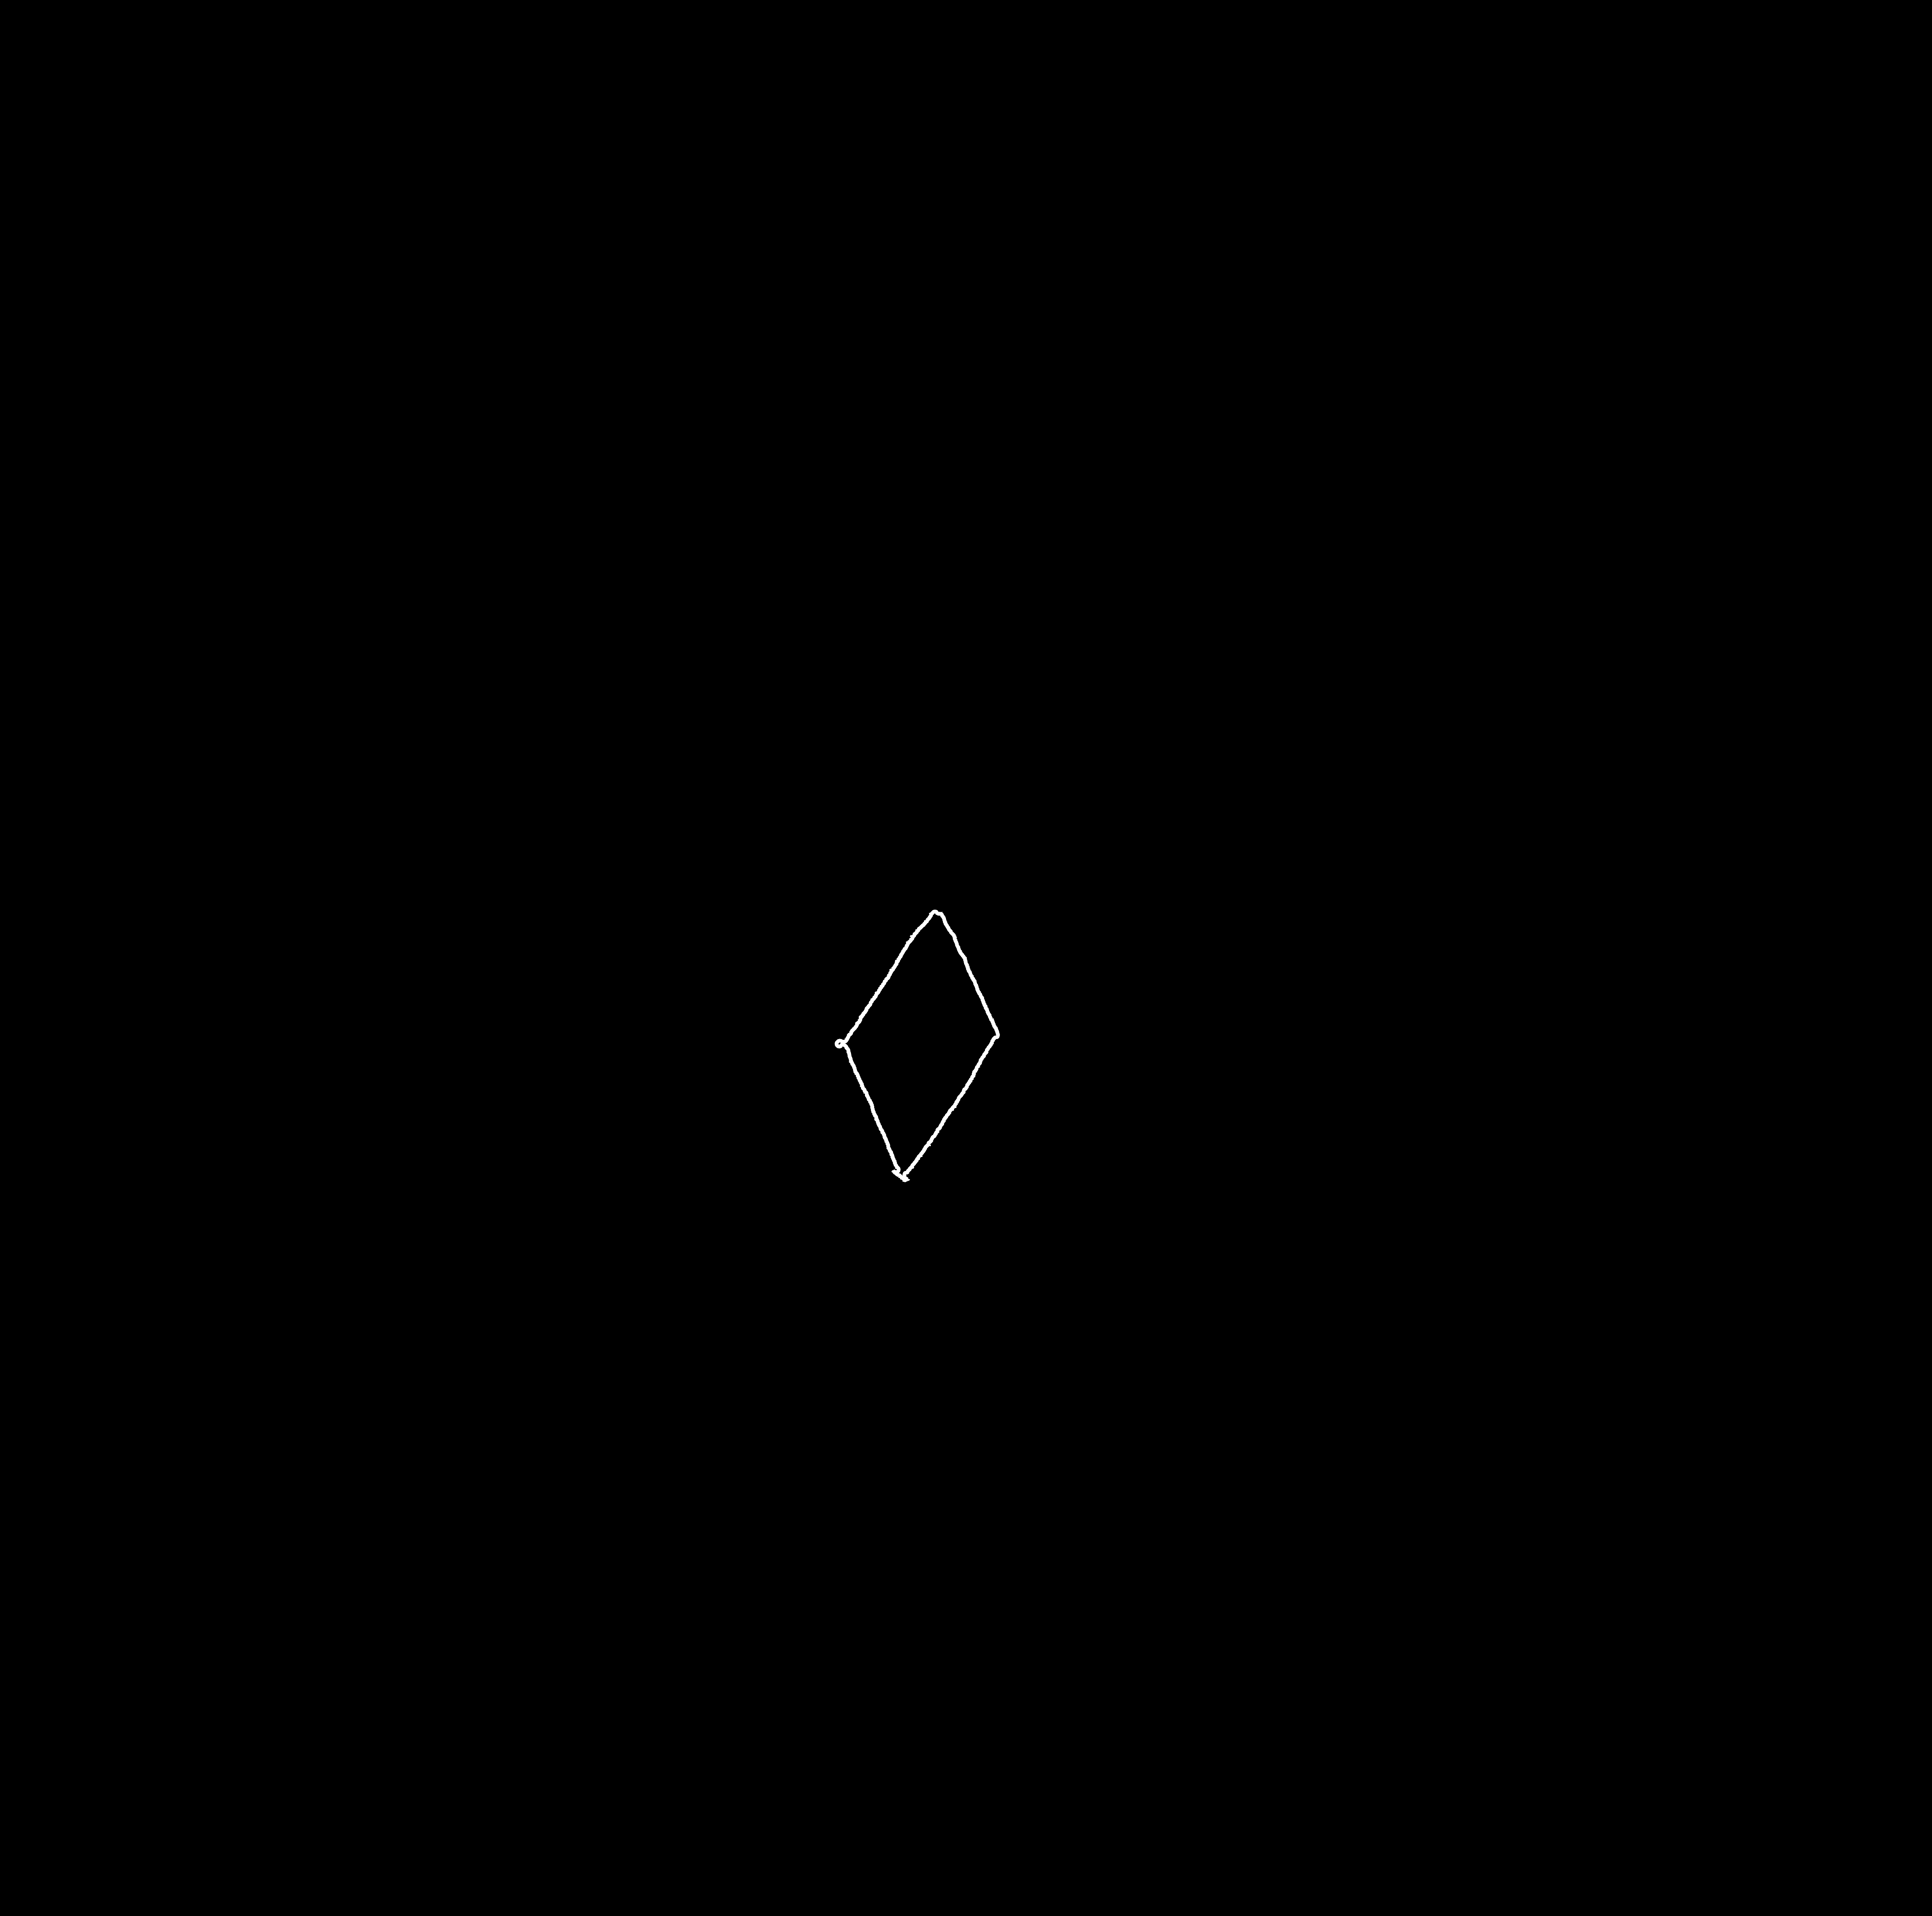
\includegraphics[angle=270, width=0.2\textwidth]{fig/diam.png}
        \label{fig:second_sub}
    }
    \caption{Detected Rectangles and Diamonds}
    \label{fig:rectNdiam}
\end{figure}
    
\subsubsection{Characterization}
    From last step, the OpenCV function  \emph{OpenCV.connectedComponentsWithStats} also returns the centroid and some statistical information as output. More specifically, the function would return the width and the height of the boundary box as well as the coordinate of the upper left corner of the boundary box. These attributes are preserved in an array for later use.

\begin{figure}[!htbp]
    \centering
    \subfigure[Circles]
    {
        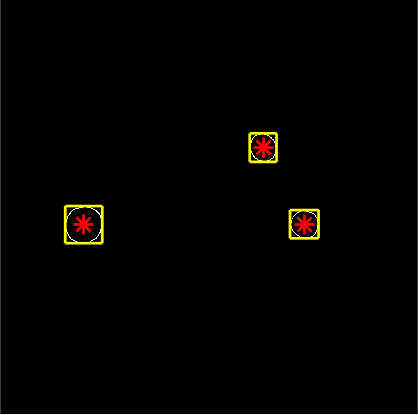
\includegraphics[angle=270, width=0.2\textwidth]{CircleBox.png}
        \label{fig:first_sub}
    }
    \subfigure[Diamonds]
    {
        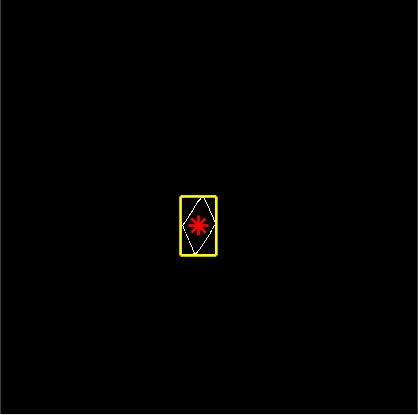
\includegraphics[angle=270, width=0.2\textwidth]{DiamondBox.png}
        \label{fig:second_sub}
    }
    \subfigure[Rectangles]
    {
        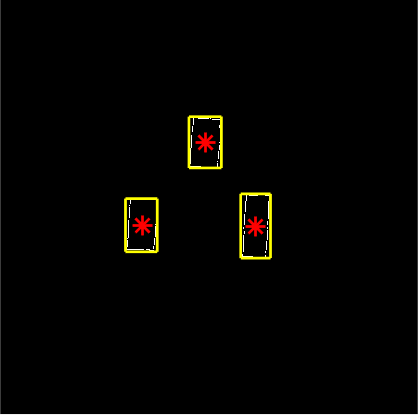
\includegraphics[angle=270, width=0.2\textwidth]{RecBox.png}
        \label{fig:first_sub}
    }
    \caption{Centroid and Boundary Box}
    \label{fig:rectNdiam}
\end{figure}

\subsubsection{Connection relationship} 
    The goal of this step is to determine the direction of arrows. Since the width, height and the upper left point of the boundary box is known, the center of the box can also be computed. By comparing the relative location of the center and the centroid of the shape, the corner that is closet to the centroid can be found. Based on the assumption that the arrows are straight, the closet corner can 
    approximate the head of the arrow, and the diagonal corner would represent the tail of the arrow. These two end points would be passed to next step, with tails and heads labeled.
    
\begin{figure}[!htbp]
    \centering
    \subfigure[Arrows centroid]
    {
        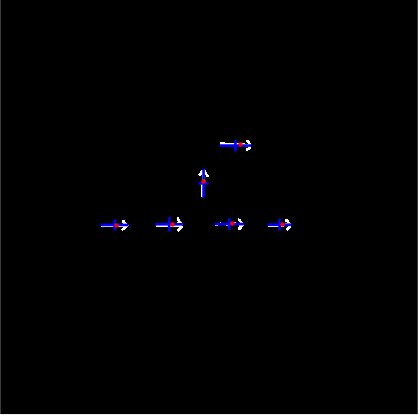
\includegraphics[angle=270, width=0.2\textwidth]{ArrowBox.png}
        \label{fig:first_sub}
    }
    \subfigure[Centroid and the four Corners]
    {
        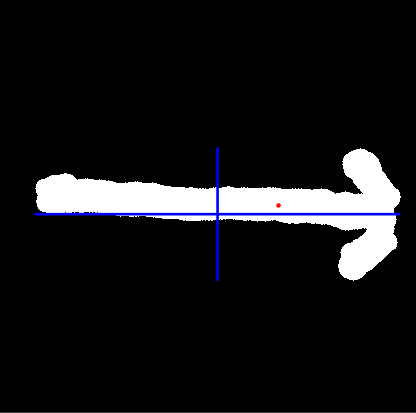
\includegraphics[angle=270, width=0.2\textwidth]{connection.png}
        \label{fig:second_sub}
    }
    \caption{Arrow Direction Determination}
    \label{fig:rectNdiam}
\end{figure}
    
\subsubsection{Reconstruction}
    In this step, we aim to find which shape for an arrow belongs to. For all diamonds, we set the four anchors on the corners of the shape. For all rectangles, anchors are set on the center of each side. Based on the two end points given from last step, we loop over all anchors, to find the closet anchor and attach the arrow on it so that the resulting flowchart would have a well-organized structure. This information collected so far would be utilized in the next section.

\subsection{Android Implementation}
We encapsulate the interfaces 
Flowchart shape is an abstract class that all other child shapes extend with. Neighbors are the other shapes that the current shape connects to and the edges represent those connected edges. For each shape, it also has an attribute called anchors which stand for a list of points an arrow can attach to. Each shape has an abstract draw method that can be customized by each child shape. As shown in figure \ref{fig: class_hierachy}
\begin{lstlisting}[language=java]
class FlowchartShape {
    List<FlowchartShape> neighbors;
    List<Edge> edges;
    List<Point> anchors;
    abstract void draw(Mat mat, 
    Scalar scalar, int thickness);
}
\end{lstlisting}

\begin{figure}[!htbp]
\begin{center}
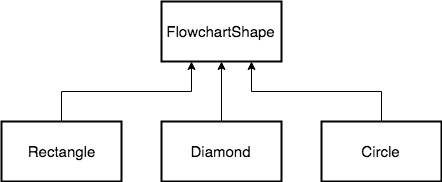
\includegraphics[scale=0.5]{class.jpg}
\caption{Class hierarchy}
\label{fig: class_hierachy}
\end{center}
\end{figure}

Rectangle, diamond and circle are three sub-classes that extend the Flowchartshape class. Each one implements helper functions and also identifies the anchor point position. When plotting the flowchart, we only need to call draw method on each shape and this polymorphism makes the flowchart plotting very convenient. 

The Graph class encapsulates the shapes and has its own draw method. In this draw method, it first draws all the shapes and then figures out how to draw arrows based on the graph data structure which is done by performing topological sort on the graph.

In order to show the real-time result while not blocking the camera frame, a separate thread is needed. When a new frame arrives, the main thread launches a background thread doing all the image processing and recognition. To avoid unnecessary computing overhead, only one background processing thread exists. Also, the result of previous processed frame is shown while the background thread is doing its job. 

As mentioned above, the flowchart recognition algorithm depends on many parameters such as binarization threshold, small region removal area and threshold in Hough transform. Therefore, those parameters should be tuned in order to achieve ideal recognition result. However, this tuning becomes very hard when we try to adjust parameters in compile time because OpenCV library is very large which makes APK installation quite slow. Thus, we also introduce the idea that we can adjust parameters in run-time. In our Android implementation, we have three buttons at the bottom of screen as shown in the figure \ref{fig: android_bottom}. The change button can switch among all those parameters and we can tune them by clicking plus and minus button. This is tuned in dynamic and can quickly show the processed result on screen. 

\begin{figure}[!htbp]
\begin{center}
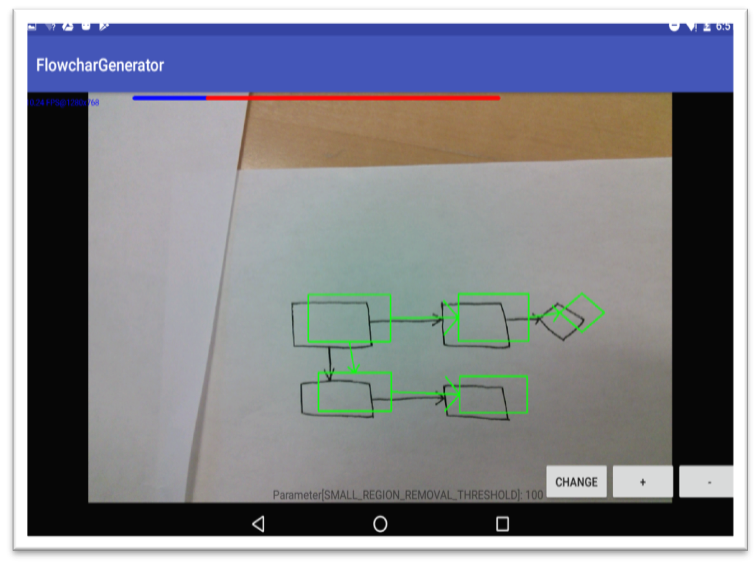
\includegraphics[scale=0.6]{android.png}
\caption{Android implementation}
\label{fig: android_bottom}
\end{center}
\end{figure}


\section{Conclusion and Future Work}

\subsection{Conclusion}
Our flowchart recognition algorithm is able to detect rectangle, diamond, circle and arrow in a flowchart in real-time. It is very user friendly, interactive and easy to use. 

\subsection{Future Work}

\subsubsection{Orientation correction}
One of very important assumption we made in the algorithm is that there should exist more rectangles in the flowchart because the correct orientation is achieved by finding the primary orientation component in the edges of rectangles. However, this is actually not generic enough in the real life conditions and would entail wrong recognition result in an extreme input. We also made an assumption that the arrow can point to any directions rather than only vertical and horizontal. This restrict us from doing correction through arrows. One solution to this problem is to make use of diamond to do orientation correction. Since the diagonals of a diamond should be perpendicular to each other, this can also indicate the flowchart orientation.
\subsubsection{Denoise}
In order to simplify the pre-processing step, we also made an assumption that the flowchart appears on a clean white paper without obvious noise. Although we have Gaussian filtering and small region removal in the algorithm, it is not enough to remove noise like book, pen or other real life objects. One easy solution can be implemented in the Android device side by asking the user to manually crop the ROI (region of interest). This can significantly improve the recognition accuracy while keeps the application user-friendly and interactive.  
\subsubsection{Testing}
One big problem in our experiment is testing. Although we manually draw a lot of flowcharts and use this test set to evaluate the algorithm, it is not enough for our real-time application. This is because even if the algorithm passed all of the test cases, it is very possible that the algorithm will fail to recognize a flowchart in the real-time settings since lighting, focus and directions all vary. Thus, a more rigorous testing should be performed to make the algorithm much more robust. One very easy way is to do module or unit test. We can implement each of intermediate step in real-time, for example, only doing binarization and see if the result meets the requirement.
\subsubsection{Export flowchart}
Our Android implementation can recognize the flowchart and plot it on the screen. A further goal is to export the flowchart so that the user can actually use it in their writing. This can be done by using third party plot packages like python graphviz and saving as a png or jpeg file.


% Can use something like this to put references on a page
% by themselves when using endfloat and the captionsoff option.
\ifCLASSOPTIONcaptionsoff
  \newpage
\fi



% trigger a \newpage just before the given reference
% number - used to balance the columns on the last page
% adjust value as needed - may need to be readjusted if
% the document is modified later
%\IEEEtriggeratref{8}
% The "triggered" command can be changed if desired:
%\IEEEtriggercmd{\enlargethispage{-5in}}

% references section

% can use a bibliography generated by BibTeX as a .bbl file
% BibTeX documentation can be easily obtained at:
% http://www.ctan.org/tex-archive/biblio/bibtex/contrib/doc/
% The IEEEtran BibTeX style support page is at:
% http://www.michaelshell.org/tex/ieeetran/bibtex/
%\bibliographystyle{IEEEtran}
% argument is your BibTeX string definitions and bibliography database(s)
%\bibliography{IEEEabrv,../bib/paper}
%
% <OR> manually copy in the resultant .bbl file
% set second argument of \begin to the number of references
% (used to reserve space for the reference number labels box)
\begin{thebibliography}{1}

\bibitem{valveny1999}
Valveny, Ernest, and Enric Martí. "Deformable template matching within a bayesian framework for hand-written graphic symbol recognition." International Workshop on Graphics Recognition. Springer, Berlin, Heidelberg, 1999.

\bibitem{Ramel1999}
Ramel, Jean-Yves, Guillaume Boissier, and Hubert Emptoz. "A structural representation adapted to handwritten symbol recognition." International Workshop on Graphics Recognition. Springer, Berlin, Heidelberg, 1999.

\bibitem{Rusinol2014}
Rusiñol, Marçal, Lluís-Pere de las Heras, and Oriol Ramos Terrades. "Flowchart recognition for non-textual information retrieval in patent search." Information retrieval 17.5-6 (2014): 545-562.

\bibitem{Morzinger2012}
Mörzinger, Roland, et al. "Visual Structure Analysis of Flow Charts in Patent Images." CLEF (Online Working Notes/Labs/Workshop). 2012.

\bibitem{Ming2018}
Ming, Wei. "Method for recognizing table, flowchart and text in document images." U.S. Patent No. 9,858,476. 2 Jan. 2018.


\end{thebibliography}

% biography section
% 
% If you have an EPS/PDF photo (graphicx package needed) extra braces are
% needed around the contents of the optional argument to biography to prevent
% the LaTeX parser from getting confused when it sees the complicated
% \includegraphics command within an optional argument. (You could create
% your own custom macro containing the \includegraphics command to make things
% simpler here.)
%\begin{biography}[{\includegraphics[width=1in,height=1.25in,clip,keepaspectratio]{mshell}}]{Michael Shell}
% or if you just want to reserve a space for a photo:

\begin{IEEEbiography}[{\includegraphics[width=1in,height=1.25in,clip,keepaspectratio]{picture}}]{John Doe}
\blindtext
\end{IEEEbiography}

% You can push biographies down or up by placing
% a \vfill before or after them. The appropriate
% use of \vfill depends on what kind of text is
% on the last page and whether or not the columns
% are being equalized.

%\vfill

% Can be used to pull up biographies so that the bottom of the last one
% is flush with the other column.
%\enlargethispage{-5in}

\section{Appendix}
The break-down of work done by each student is listed as follows.
\begin{itemize}
    \item Qian Yu designed data structure and realized Android device implementation
    \item Rao Zhang implemented the steps from image binarization (step 2) to shape classification (step 6).
    \item Tien-Ning Hsu collaborated work from shape classification (step 6) to component connection (step 8).
    \item Zheng Lyu collaborated work from shape classification (step 6) to component connection (step 8).
\end{itemize}



% that's all folks
\end{document}


